\documentclass[
	%parspace, % Add vertical space between paragraphs
	%noindent, % No indentation of first lines in each paragraph
	%nohyp, % No hyphenation of words
	%twoside, % Double sided format
	%draft, % Quicker draft compilation without rendering images
	%final, % Set final to hide todos
]{elteikthesis}[2025/04/26]

% The minted package is also supported for source highlighting
% See elteikthesis_minted.tex for example
%\usepackage[newfloat]{minted}

% Document's metadata
\title{Lidar-Based map-observation Localization Module for Autonomous Navigation} % title
\date{2025} % year of defense

% Author's metadata
\author{Eliyas Kidanemaraim Abraha}
\degree{Bachelor of Science}

% Superivsor(s)' metadata
\supervisor{Zoltan Istenes} % internal supervisor's name
\affiliation{Assistant Professor} % internal supervisor's affiliation
\extsupervisor{Mohammad Aldibaja} % external supervisor's name
\extaffiliation{Assistance Professor} % external supervisor's affiliation

% University's metadata
\university{Eötvös Loránd University} % university's name
\faculty{Faculty of Informatics} % faculty's name
\department{IFROS} % department's name
\city{Budapest} % city
\logo{elte_cimer_szines} % logo

% Add bibliography file
\addbibresource{elteikthesis.bib}

% The document
\begin{document}

% Set document language
%\documentlang{hungarian}
\documentlang{english}

% List of todos (not in the final document)
%\listoftodos[\todolabel]

% Title page (mandatory)
\maketitle

% Topic declaration page (mandatory) - can also be attached instead
%\includepdf{topicdeclaration.pdf}

% Table of contents (mandatory)
\tableofcontents
\cleardoublepage

% Main content
\chapter{Introduction}
\label{ch:intro}

\section{Motivation}
High-precision and reliable localization is crucial for autonomous vehicles and robots, as it directly affects tasks like path planning, obstacle avoidance, and other repetitive missions \cite{kim2018stereo}. Typically, positioning relies on Global Navigation Satellite Systems (GNSS) and Inertial Navigation Systems (INS), which complement each other. GNSS can provide absolute position without drift especially when using differential signals while INS delivers frequent updates to track movement\cite{carvalho1997optimal}. However, in urban areas with tall buildings or indoor environments, GNSS signals can be blocked or distorted, and INS alone may accumulate significant drift over time\cite{liu2019segmentation}. Moreover, these systems do not inherently provide information about the surrounding environment.

To address such limitations, researchers have adopted onboard sensors like LiDAR, monocular cameras, and stereo cameras. One widely used method is Simultaneous Localization and Mapping (SLAM), which enables a robot to estimate its position in a completely new environment without needing a prior map. While SLAM is flexible and powerful, it can drift if loop closures are infrequent or the robot cannot revisit known areas to correct its estimates.

An alternative that improves accuracy and stability is map-based localization, where a pre-built map (created beforehand by SLAM, GNSS-based surveys, or other methods) is used as a global reference \cite{levinson2007mapbased}. In this approach, the robots’s current sensor data such as LiDAR scans are matched against the detailed information in the map to determine its position. This matching process helps minimize drift and provides robust localization, even in environments where GNSS signals are unavailable or unreliable. Once the map is constructed, indoor and outdoor autonomous systems can repeatedly use it to perform their tasks more reliably, whether that involves delivering goods, patrolling a facility, or navigating urban streets. As a result, map-based localization is considered an indispensable component of future autonomous navigation, especially when consistent high accuracy and global reference information are required.


Despite its advantages, map-based localization poses several challenges.First,real-time performance requires efficient management of high-resolution 3D maps and the use of fast, precise scan-to-map matching algorithm for accurate pose estimation. Second, integrating local motion estimation (e.g., via LiDAR-Inertial Odometry) with global map alignment must be handled carefully to ensure both consistency and computational feasibility. Finally, the presence of dynamic objects and adverse environmental conditions further complicates the localization pipeline.


This thesis addresses these challenges by proposing a hybrid system that combines real-time LiDAR-Inertial Odometry (FAST-LIO2), efficient map-matching via multithreaded NDT (NDT-OMP), and a sliding-window factor graph fusion approach. The system dynamically loads submaps around the robot based on a configurable radius, allowing scalable scan-matching while maintaining global consistency.In addition, a learning-based object detection module identifies and removes dynamic objects from the LiDAR scans, further enhancing robustness. Together, these components form a real-time, accurate, and robust localization framework tailored for large-scale, \textbf{semi-dynamic} environments.

\section{Objective}

The primary objective of this thesis is to develop a real-time, LiDAR-based localization framework that achieves both high-frequency motion estimation and drift-free global consistency in large-scale environments. This is accomplished by integrating LiDAR-Inertial Odometry with map-based scan matching, and fusing them through a computationally efficient sliding-window factor graph.
\begin{itemize}
    \item To integrate a robust LiDAR-Inertial Odometry(LIO) module using FAST-LIO2, capable of providing real-time pose estimates by tightly coupling LiDAR and IMU data.
    \item To develop a scan-to-map matching module by integrating a multithreaded Normal Distributions Transform (NDT-OMP) algorithm, enabling real-time alignment of incoming LiDAR scans with a pre-built 3D point cloud map. 
    % This approach leverages the robustness of NDT for point cloud registration while utilizing parallel processing to maintain computational efficiency.

   
    \item To fuse LiDAR-Inertial Odometry(LIO) and map matching results using a sliding-window factor graph optimization approach, enabling efficient, bounded optimization that retains local consistency while discarding outdated states.
    %\item To integrate a learning-based dynamic object detection module into the LiDAR processing pipeline.%
     \item To design and implement a grid-based submap management system that loads only the relevant local tiles within a configurable radius of the robot’s position and incrementally replaces out-of-range tiles without reloading the full map.
    \item To evaluate the proposed system on benchmark datasets and custom scenarios, measuring performance in terms of localization accuracy, computation time, memory usage, and robustness under varying environmental conditions.
\end{itemize}
% \section{Problem Statement}
\section{Research Questions}

The primary questions guiding this research are:
\begin{enumerate}
	\item How can LiDAR-Inertial odometry(FAST-LIO2) and NDT-based map matching be effectively fused to enhance real-time localization accuracy and robustness?
    \item How does integrating a pre-built map improve the accuracy and robustness of LiDAR-based localization in GNSS-denied environments?
    % \item Which scan-to-map matching techniques offer the best trade-off between accuracy and computational efficiency for large-scale or dynamic environments?
    % \item What role does sensor fusion (e.g., LiDAR-inertial, LiDAR-wheel odometry) play in enhancing the reliability of map-based localization?
    % \item How can we optimize both map representation and scan processing to ensure scalable and efficient localization?
    
    \item What is the impact of dynamic submap loading and grid-based map management on computational performance and scalability?
    
    \item Does the proposed localization method     maintain accurate localization in feature sparse and noisy environmental condition?
    
    % \item How can LiDAR-Inertial odometry (FAST-LIO2) and multithreaded NDT-based scan matching be effectively fused to achieve both accuracy and real-time performance?
    % \item How does sliding-window factor graph optimization compare to full graph smoothing in terms of runtime and pose consistency?
\end{enumerate}
\section{Scope and limitations}
\subsection{Scope}
The proposed localization system is designed for real-time operation in diverse environments, including indoor spaces, outdoor areas, and urban environments. It assumes the availability of a high-resolution 3D LIDAR map of the operation environment. The system provides accurate pose estimation by fusing LIDAR-Inertial Odometry with scan-to-map matching, and its particularly suited scenarios where GNSS is unreliable or unavailable.
\subsection{Limitations}
\begin{itemize}
    \item The system does not perform global localization (i.e., it cannot determine an unknown initial pose within the map). It assumes the robot starts with a known or approximated initial position close to its true location.
    \item The approach relies entirely on a pre-built map; it does not perform simultaneous mapping (SLAM) or update the map during operation.
    \item Highly dynamic environments or areas with significant structural changes may affect scan matching accuracy and overall system.
\end{itemize}


%\section{Methodology overview}
% \section{Contribution of the thesis}
% \begin{enumerate}
%     \item  A robust framework that integrates LiDAR scans with a pre-built map to reduce drift and improve global consistency.
%     \item Comparative Study of Scan-Matching Techniques: An in-depth evaluation of multiple algorithms (e.g., ICP variants, Normal Distributions Transform) in terms of accuracy and efficiency.
%     \item Sensor Fusion Integration: A demonstration of how additional sensors (e.g., IMU, wheel encoders) can enhance localization stability and resilience.
%     \item Scalability Insights: Guidelines and best practices for handling large-scale maps to maintain real-time performance.
% \end{enumerate}

\section{Overview of the thesis structure}
\begin{itemize}
    \item Chapter 2 – Literature Review: Provides a comprehensive overview of state-of-the-art LiDAR-based localization techniques, including LiDAR–Inertial Odometry, SLAM, map-based localization, scan-matching algorithms, sensor-fusion methods, and learning-based 3D dynamic-object removal.
    
    \item Chapter 3 – Methodology: Describes the design of the proposed system, including each module, the integration flow, and technical implementation details.
 	   \item Chapter 4 - Experimental setup and results: Presents experimental evaluations, including performance metrics and comparisons with baseline approaches.
    \item Chapter 5 – Discussion: Interprets the findings, discusses limitations, and addresses how the proposed system meets the research objectives.
    \item Chapter 6 - Conclusion and future work: Summarizes key contributions, discusses possible improvements, and proposes directions for further research.
\end{itemize}

% The rest of the thesis is organized as follows. Chapter 2 overviews the related
% literature, including a brief description of the selected reference LIO-SAM frame-
% work. The proposed method, including exploration and localization, is described
% in Chapter 3. Experimental results are reported in Chapter 4 and discussed in
% Chapter 5. Finally, the thesis is concluded in Chapter 6.





\cleardoublepage
\chapter{Litreature Review}
\label{ch:intro}
\section{Overview of Relevant Literature}
This section provides an overview of the foundational literature relevant to the design and development of the proposed localization system. It reviews key concepts and techniques in LiDAR and LiDAR-Inertial Odometry, SLAM, map-based localization, point cloud registration, and dynamic object detection using 3D LiDAR data.

\subsection{LiDAR and LiDAR-Inertial Odometry Techniques}
Localization is a crucial capability for mobile robots, referring to the process of determining the robot’s position and orientation in a given environment. Early attempts at localization depended heavily on wheel encoders, commonly known as wheel odometry, but this method suffered from significant drift whenever the wheels slipped or the ground was uneven \cite{MohamedOdometry}. As robotics advanced, researchers explored range sensors and visual sensors to improve motion estimation \cite{WangVisionSurvey}. At the same time, algorithms like Iterative Closest Point (ICP) emerged, enabling the alignment of consecutive scans and sparking a separate stream of research in range sensor‐based odometry \cite{BeslICP1992}.

Building on these ideas, LiDAR‐only odometry gained popularity due to LiDAR’s immunity to lighting changes and ability to capture dense 3D data. One key approach uses straightforward scan matching via ICP \cite{BeslICP1992}, but such methods can struggle in environments with few unique geometric features. To address this, feature-based systems extract distinctive cues from each LiDAR scan, as demonstrated in LOAM \cite{ZhangSinghLOAM2014}, where sharp edges and planar surfaces guide the matching process. While LiDAR‐only odometry can produce accurate short‐term estimates, it may drift over time if the robot moves rapidly or the environment is mostly repetitive.

To reduce long‐term drift, many researchers incorporate IMU (Inertial Measurement Unit) data, resulting in what is called LiDAR–Inertial Odometry (LIO). In a loosely coupled setup, LiDAR and IMU each compute their own pose, and then a higher‐level filter (like an Extended Kalman Filter) merges these estimates \cite{TangLooselyCoupled}. This approach is easier to design because the LiDAR odometry module and the IMU integration module work somewhat independently. However, the separate modules might not fully exploit each other’s measurements.

By contrast, tightly coupled designs feed raw IMU data directly into the LiDAR optimization. For instance, LIO-SAM employs a factor graph where both LiDAR and IMU preintegration factors are updated in the same framework, allowing more constraints to be used in each calculation \cite{ShanEtAlLIOSAM2020}. As graph‐based LiDAR–inertial odometry solutions grew more complex and demanding, researchers began exploring filter‐based methods built around the Kalman filter. One notable example is LINS \cite{lins}, which uses an iterated Error State Kalman filter (iESKF) to speed up pose estimation; however, it still faces performance bottlenecks when dealing with large numbers of LiDAR points, since computing the Kalman gain for every point can be costly. In response, FAST‐LIO \cite{xuFastLIO2021} introduced a more efficient Kalman gain calculation that significantly lowers this overhead. Later, As shown in Figure~\ref{fig:fast_lio2_architecture} FAST‐LIO2 \cite{xuFastLIO2} expanded on that approach by completely removing the feature extraction step and matching raw LiDAR points directly to the map. To accelerate nearest‐neighbor queries, it employs a specialized data structure called an ikd‐Tree, allowing the system to achieve both high accuracy and even faster run.

\begin{figure}
    \centering
    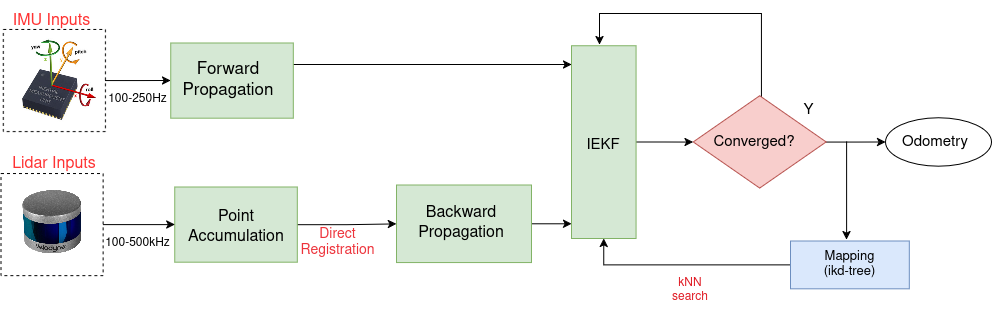
\includegraphics[width=1 \linewidth]{images/fast_lio.drawio.png}
    \caption{Architecture of FAST-LIO2: A tightly coupled LiDAR-Inertial Odometry 
    	\cite{xuFastLIO2}}
    \label{fig:fast_lio2_architecture}
\end{figure}

Due to its high computational efficiency, accuracy, and real-time capability, FAST-LIO2 is adopted in this thesis as the LiDAR-Inertial Odometry (LIO) front-end. Its design aligns with the system’s objective to maintain high-frequency odometry while minimizing drift, providing a solid foundation for downstream scan-to-map correction and graph-based fusion.

\subsection{SLAM and Loop Closure-Based Localization}
Moving beyond pure odometry, SLAM (Simultaneous Localization and Mapping) takes an extra step by adding loop closure mechanisms to maintain global consistency \cite{cadena2016past}. While LiDAR–Inertial Odometry can reduce local drift, it remains prone to cumulative error over long distances if no global corrections are made. By detecting revisits to previously mapped areas, a full SLAM pipeline like Google Cartographer (for 2D LiDAR) \cite{hess2016real} or other graph‐based back ends \cite{grisetti_gmapping,} refines the entire trajectory, resulting in notably higher accuracy.Recent SLAM systems like MOLA slam \cite{blanco2025mola_lo} and KISS-ICP\cite{kiss2025arxiv} have further advanced LiDAR-based localization by improving loop closure detection and trajectory optimization for large-scale environments. However, these systems carry greater computational cost and design complexity, since maintaining a global graph or submap structure calls for advanced data management.

SLAM inherently relies on loop‐closure events or prior constraints to limit its global drift; if these loop closures are sparse or absent over a long trajectory, the system can still accumulate significant positioning errors \cite{grisetti_gmapping, cadena2016past}. That limitation underscores the motivation for map‐based localization, in which an existing map is used to provide absolute constraints and reduce drift, even in lengthy or repetitive environments where loop closures are not guaranteed.

\subsection{Localization Using Prior Maps}
Estimation of the position of a sensor on a map is essential for navigation systems. While several
kinds of map representations are used, depending on the use scenario 3D point cloud maps are among the most popular representations owing to their simplicity and expressiveness.\cite{koide2024tightly}Because constructing a point cloud map is relatively easy with recent precise range sensors and mapping algorithms, point cloud maps are used for a wide range of applications, from indoor service robots to outdoor driving of autonomous vehicles.


Monte Carlo Localization (MCL) is a well-established probabilistic technique for 2D map-based localization~\cite{thrun2005probabilistic}. It excels in handling non-linear and non-Gaussian systems, offering robustness to ambiguous observations and multi-modal distributions. However, its application in 3D localization is rare due to the exponential increase in the number of particles required to represent the full 6-DoF state space. This makes real-time use in point cloud-based 3D environments computationally prohibitive

Multiple recent works highlight the potential of map-aided localization for achieving robust and precise vehicle pose estimation.\cite{Levinson2007MapBased} propose building a 2D road-surface reflectivity map from lidar data, then using real-time lidar scan correlation against this map to localize within a few decimeters in busy urban areas.Similarly,\cite{liu2019segmentation} adopt a detailed segmentation approach: each incoming lidar frame is broken down into ground, curb, edge, and surface features,which are then aligned with a prior feature map; the refined estimates are further fused with a MEMS-IMU for centimeter-level accuracy at high frequency.

By contrast,\cite{Lin2021Autonomous} utilize stereo-based “visual point cloud” maps, avoiding LiDAR hardware yet involving dense stereo matching for both the offline (map) and online (frame) steps. Their system then registers these point clouds via normal distribution transform (NDT). While it lowers sensor costs, it adds a heavy stereo workload and remains susceptible to lighting or texture issues. The authors also report that deviations can occur at sharp turns, albeit these are later corrected. Finally, \cite{Rozenberszki2020LOL} integrate LOAM odometry with a global segment-based prior map (via SegMap) for re-localization when drift accumulates. The system occasionally triggers place recognition in the global map, confirms geometry with RANSAC, then refines the pose using fine-grained ICP.

By contrast, \cite{Lin2021Autonomous} utilize stereo-based “visual point cloud” maps, avoiding LiDAR hardware yet involving dense stereo matching for both the offline (map) and online (frame) steps. Their system then registers these point clouds via normal distribution transform (NDT). While it lowers sensor costs, it adds a heavy stereo workload and remains susceptible to lighting or texture issues.The authors also report that deviations can occur at sharp turns, albeit these are later corrected. Similarly, \cite{kim2018stereo} propose a stereo vision localization method within 3D LiDAR maps by extracting visual features in the Bird’s-Eye View (BEV) domain and matching them to the LiDAR map. Finally, \cite{Rozenberszki2020LOL} integrate LOAM odometry with a global segment-based prior map (via SegMap) for re-localization when drift accumulates. The system occasionally triggers place recognition in the global map, confirms geometry with RANSAC, then refines the pose using fine-grained ICP.


Together, these works illustrate the diversity of map-based localization strategies, but many are constrained by computational inefficiency, dependence on handcrafted or road-specific map features, and limited scalability or adaptability to dynamic and degraded environments. This underscores the need for a more efficient, generalizable, and real-time-capable localization framework.

\subsection{Point Cloud Registration Techniques}
Point cloud registration is a key technique in LiDAR-based localization, used to align a current LiDAR scan with a prior map to estimate the sensor’s pose. The classic Iterative Closest Point (ICP) algorithm performs this by minimizing distances between matched point pairs across the two clouds. While ICP is conceptually simple, it suffers from sensitivity to noise, poor initial alignment, and local minima, making it unreliable for large-scale or noisy environments \cite{BeslICP1992}.

To address these limitations, the Normal Distributions Transform (NDT) was proposed by \cite{biber2003ndt} and
further elaborated in subsequent research\cite{magnusson2007ndt}.  NDT offers a compact representation
of surfaces by converting point clouds into a set of local probability density functions
(PDFs), each characterizing a surface section.Instead of relying on discrete point matches, NDT represents the map as a grid of voxels, each containing a Gaussian distribution that models the local geometry. Scan points are registered by maximizing their likelihood under these distributions. This makes NDT more robust to outliers, partial overlaps, and noisy measurements.

Modern implementations such as NDT-OMP further improve runtime performance through multi-threading, enabling real-time scan-to-map matching in large-scale environments \cite{koide2019portable}. Due to its robustness and efficiency, NDT is widely used in autonomous driving and is adopted in this thesis for scan-matching against a pre-built point cloud map.

\subsection{Dynamic Object Removal Techniques}

In LiDAR-based localization, scan-matching techniques are widely employed to align real-time sensor data with a pre-built static map. However, dynamic objects such as moving vehicles, pedestrians, and cyclists introduce discrepancies between the current point cloud and the static reference. These inconsistencies can significantly degrade localization performance, leading to pose drift, poor convergence, or failure in highly dynamic environments.

To enhance the reliability of scan-matching, dynamic object removal has been introduced as a crucial preprocessing step. Early methods, including Euclidean clustering, geometric filtering, and background subtraction, identified dynamic elements based on heuristics such as size, shape, or temporal consistency \cite{liu2019segmentation,koide2019portable} . Although computationally efficient, these approaches often struggle in cluttered or semi-structured environments, resulting in high false positive rates and poor generalization.
\begin{figure}
	\centering
	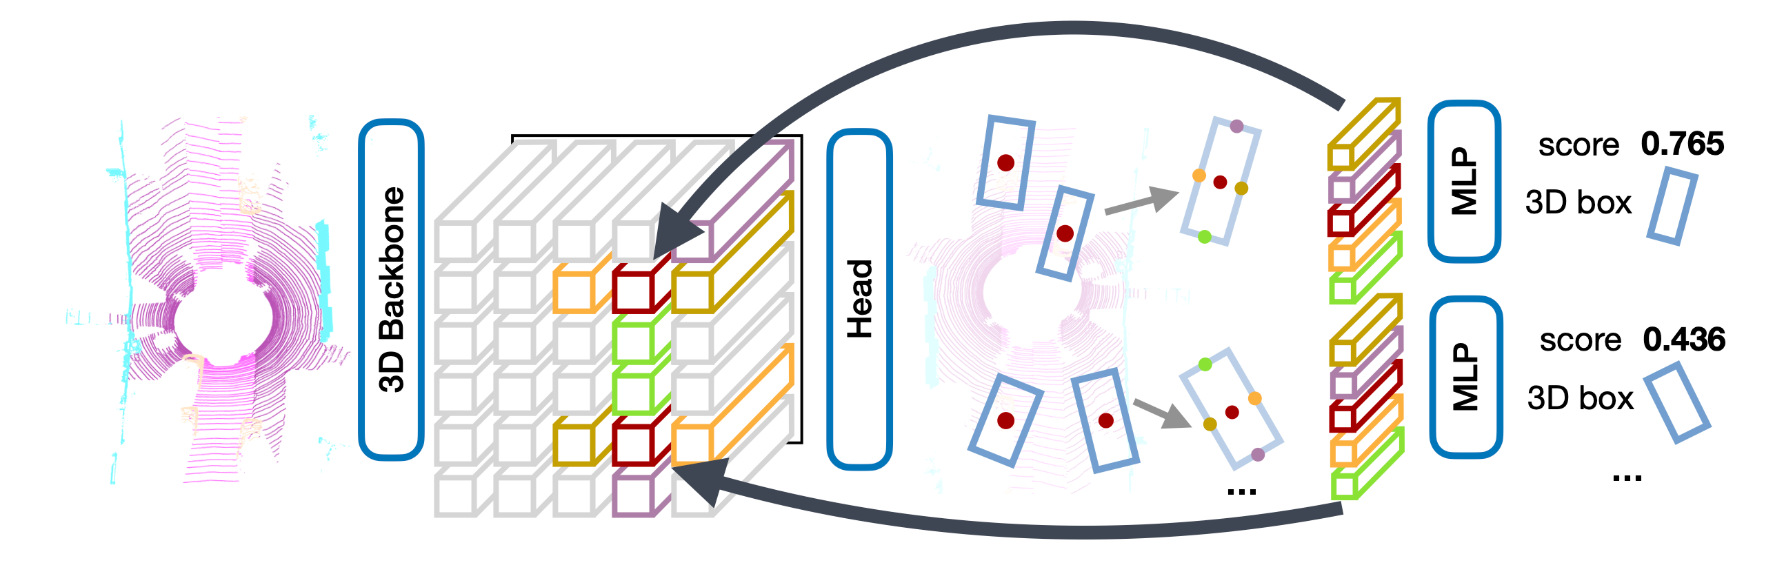
\includegraphics[width=1
	\linewidth]{images/center_point2.png}
	\caption{Overview of CenterPoint 3d object detection framework.  \cite{yin2021center}}
	\label{fig:Overview-CenterPoint }
\end{figure}
Recent advancements leverage deep learning-based 3D object detection models such as PointPillars\cite{lang2019pointpillars}, SECOND \cite{yan2018second}, and CenterPoint \cite{yin2021center} to semantically identify dynamic agents. By predicting 3D bounding boxes for known classes, these models enable precise removal of dynamic objects, preserving static features critical for accurate localization.

Among these, CenterPoint\cite{yin2021center}has emerged as a state-of-the-art solution. It employs a center-based detection paradigm over voxelized LiDAR input and achieves high accuracy on large-scale datasets such as nuScenes\cite{caesar2020nuscenes}, making it particularly suitable for real-time dynamic object filtering.

CenterPoint follows a two-stage architecture\cite{yin2021center}. First, the raw LiDAR point cloud is voxelized into a sparse 3D tensor, allowing efficient processing by sparse convolutional neural networks. A backbone network typically based on PointPillars \cite{lang2019pointpillars} or SECOND\cite{yan2018second} extracts spatial features while maintaining the geometric structure of the environment. These features are projected onto a Bird’s-Eye View (BEV) representation, preserving spatial relationships and enabling faster 2D convolutional operations. In the second stage, a keypoint-based detection head predicts object centers by generating a center heatmap over the BEV feature map. Following center localization, the model regresses the full set of object attributes, including 3D bounding box dimensions, orientation (yaw angle), velocity, and semantic class label. This decoupled center-to-attribute approach simplifies the detection task and enhances robustness against small, distant, or partially occluded objects, as illustrated in Figure \ref{fig:Overview-CenterPoint }.Due to its high detection accuracy and real-time inference capability, CenterPoint is adopted in this work as the dynamic object detection module.


\section{Theoretical Background }
% \subsection{Point-Cloud Registration}

\subsection{Normal Distributions Transform (NDT)}
\label{sec:Normal Distributions Transform}

% \paragraph{Mathematical Formulation}
The NDT algorithm begins by subdividing the space occupied by a scan into discrete grid cells---squares in 2D or cubes in 3D. A PDF is calculated for each cell based on the distribution of points within that cell. Each PDF describes how points within the cell are likely generated, assuming the points result from a multivariate normal random process. The probability density function for a cell is defined as:

\begin{equation}
p(\mathbf{x}) = \frac{1}{(2\pi)^{D/2}|\mathbf{\Sigma}|^{1/2}} \exp\left(-\frac{1}{2}(\mathbf{x}-\mathbf{\mu})^T\mathbf{\Sigma}^{-1}(\mathbf{x}-\mathbf{\mu})\right)
\end{equation}

where $\mu$ and $\Sigma$ denote the mean vector and covariance matrix of the reference of the scan surface points within the cell where x lies. The mean and the covariance are computed as 

\begin{equation}
\mathbf{\mu} = \frac{1}{m} \sum_{k=1}^{m} \mathbf{y}_k
\end{equation}

\begin{equation}
\mathbf{\Sigma} = \frac{1}{m - 1} \sum_{k=1}^{m} (\mathbf{y}_k - \mathbf{\mu})(\mathbf{y}_k - \mathbf{\mu})^T
\end{equation}

where $y_k = 1 ,..., m  \ldots$  are the positions of the reference scan points contained in the cell.

This probabilistic representation gives a piecewise smooth surface approximation with continuous derivatives, capturing the local surface position, orientation, and smoothness effectively.

% \paragraph{Scan Registration Using NDT}
When applying NDT for scan registration, the objective is to determine the pose of the current scan that maximizes the likelihood that scan points align with the reference map surface.The parameters to be optimised; that is, the rotation and translation of the pose estimate of the current scan, can be encoded in a vector $\vec{p}$. The current scan is represented as a point cloud $X = \{\vec{x}_1, \dots, \vec{x}_n\}$. Assume that there is a spatial transformation function $T(\vec{p}, \vec{x})$ that moves a point $\vec{x}$ in space by the pose $\vec{p}$.Given some PDF $\vec{p}$ for scan points, the optimal pose  maximizes the likelihood function:


\begin{equation}
\Psi = \prod_{k=1}^{n} p(T(\mathbf{p}, \mathbf{x}_k))
\end{equation}

or equivalently minimizes the negative log-likelihood of $\Psi$

\begin{equation}
-\log \Psi = -\sum_{k=1}^{n} \log p(T(\mathbf{p}, \mathbf{x}_k))
\end{equation}

    % \begin{algorithm}[htbp]
    % \caption{Scan Registration using Normal Distributions Transform (NDT)}
    % \label{alg:ndt_registration}
    % \begin{algorithmic}[1]
    %     \Require Current scan point cloud $X = \{\vec{x}_1, \dots, \vec{x}_n\}$, Reference map represented by PDFs in grid cells.
    %     \Ensure Optimized pose vector $\vec{p}$ minimizing negative log-likelihood:
    %     \[
    %     -\log \Psi = -\sum_{k=1}^{n} \log p\left(T(\vec{p}, \vec{x}_k)\right)
    %     \]
    
    %     \State \textbf{Initialize} pose estimate $\vec{p}$
    %     \Repeat
    %     \State Compute objective function:
    %         \[
    %         score(\vec{p}) = -\sum_{k=1}^{n}\log p\left(T(\vec{p}, \vec{x}_k)\right)
    %         \]
    %     \State Compute gradient and Hessian:
    %         \[
    %         \vec{g}(\vec{p}) = \frac{\partial\, score(\vec{p})}{\partial\,\vec{p}}, \quad H(\vec{p}) = \frac{\partial^2\, score(\vec{p})}{\partial\,\vec{p}^2}
    %         \]
    %     \State Compute pose update using Newton's method:
    %         \[
    %         \Delta\vec{p} = -H(\vec{p})^{-1}\vec{g}(\vec{p})
    %         \]
    %     \State Determine step length $\alpha$ (line search):
    %         \[
    %         \alpha = \arg\min_{\alpha} score(\vec{p} + \alpha \Delta\vec{p})
    %         \]
    %     \State Update pose:
    %         \[
    %         \vec{p} \leftarrow \vec{p} + \alpha \Delta\vec{p}
    %         \]
    %     \Until{convergence criterion satisfied or maximum iterations reached}
    %     \State \Return final optimized pose $\vec{p}$
    % \end{algorithmic}
    % \end{algorithm}

The primary distinction between 2D and 3D NDT algorithms resides in the spatial transformation function and its partial derivatives. In 2D, rotations are represented by a single angle, while in 3D, rotations require more complex representations( rotation matrices or quaternion representations).

\subsection{Sensor Fusion Approaches}

\subsubsection{Filtered Based Approaches}
Filtering-based sensor fusion recursively estimates a system’s state using two main phases: a prediction step (where the state is propagated using a motion model) and an update step (where incoming sensor measurements refine that prediction) \cite{thrun2005probabilistic}.This real-time, sequential estimation framework is widely employed in robotics to handle noisy sensors while maintaining tractable computational load. Nonetheless, large global corrections or loop closures can be challenging to incorporate without more advanced smoothing or factor-graph techniques\cite{cadena2016past}.

\begin{enumerate}
    \item \textbf{Extended Kalman Filter(EKF) }extends the linear Kalman Filter \cite{kalman1960new} to handle nonlinear systems by linearizing the motion and measurement models around the current estimate. It is widely used due to its computational simplicity, although linearization can degrade accuracy in highly nonlinear settings~\cite{thrun2005probabilistic}.
    
    % Let $\mathbf{x}_k$ denote the state at time $k$, and 
    % $\hat{\mathbf{x}}_{k|k-1}$ be the predicted mean. 
    
    % The \emph{prediction} step is
    %     \begin{equation}
    %     \hat{\mathbf{x}}_{k|k-1} = \mathbf{f}\bigl(\hat{\mathbf{x}}_{k-1|k-1}, \mathbf{u}_{k}\bigr), \quad
    %     \mathbf{P}_{k|k-1} = \mathbf{F}_k \,\mathbf{P}_{k-1|k-1}\,\mathbf{F}_k^T + \mathbf{Q}_k,
    %     \end{equation}
    %     where $\mathbf{F}_k$ is the Jacobian of $\mathbf{f}$ w.r.t.\ the state, $\mathbf{Q}_k$ is the process noise covariance, and $\mathbf{u}_k$ is any control input. 
        
    % The \emph{update} step uses a measurement model $\mathbf{h}$ is 
    %     \begin{equation}
    %     \mathbf{K}_k = \mathbf{P}_{k|k-1} \,\mathbf{H}_k^T 
    %     \bigl(\mathbf{H}_k\,\mathbf{P}_{k|k-1}\,\mathbf{H}_k^T + \mathbf{R}_k\bigr)^{-1}
    %     \end{equation}
    %     \begin{equation}
    %         \hat{\mathbf{x}}_{k|k} = \hat{\mathbf{x}}_{k|k-1} + \mathbf{K}_k 
    %         \bigl(\mathbf{z}_k - \mathbf{h}(\hat{\mathbf{x}}_{k|k-1})\bigr),
    %     \end{equation}
        % where $\mathbf{H}_k$ is the Jacobian of $\mathbf{h}$, $\mathbf{R}_k$ is measurement noise covariance, and $\mathbf{z}_k$ is the sensor measurement. 
      
    \item \textbf{Error State Kalman Filter(ESKF)} focuses on estimating the deviation between a nominal trajectory and the true state~\cite{mourikis2007multi}. A separate routine generates a continuous nominal estimate, while the ESKF maintains small error states for position, orientation, and sensor biases:
\begin{equation}
\delta \mathbf{x}_k = \mathbf{x}_k - \hat{\mathbf{x}}_{k}^{\text{nominal}}.
\end{equation}
By filtering only $\delta \mathbf{x}_k$, it improves numerical stability in rotation and bias terms, and is particularly effective for high-rate IMU fusion (e.g., in FAST-LIO~\cite{xuFastLIO2021} or LINS~\cite{lins}). Major loop closures or global corrections remain difficult in a strictly forward-update framework~\cite{cadena2016past}.

    \item \textbf{Unscented Kalman Filter(UKF)} avoids explicit Jacobian linearization by employing a deterministic sampling approach (sigma points)~\cite{julier1997new}. A set of points $\{\boldsymbol{\chi}_i\}$ is chosen around the mean and propagated through the nonlinear functions $\mathbf{f}$ and $\mathbf{h}$. The resulting transformed set describes the posterior distribution more accurately than a simple first-order expansion. While the UKF handles significant nonlinearities better than the EKF, it can be more computationally demanding~\cite{thrun2005probabilistic}.

    
\end{enumerate}
% \subsubsection{Factor Graph--Based Sensor Fusion}

% Factor graphs are a powerful framework for multi-sensor fusion in robotics, enabling the simultaneous estimation of all states across time. Unlike filtering approaches such as the Extended Kalman Filter (EKF), factor graphs formulate state estimation as a global optimization problem, naturally handling nonlinearities, drift correction, and loop closures~\cite{cadena2016past, dellaert2017factor}.

% Factor graphs are an undirected bipartite alternative that separate variable nodes (e.g., poses) from factor nodes (e.g., constraints)~\cite{kschischang1998factor}.Figure 2.2 shows a factor graph commonly used in localization and sensor fusion. The green nodes represent robot poses (state variables) over time, while red nodes indicate measurement constraints (e.g., sensor observations) and blue nodes represent motion constraints (e.g., from odometry or IMU). Each factor connects to the relevant states it constrains, forming a graph structure that allows for efficient joint optimization of the trajectory. They explicitly model the factorization of the joint distribution:
% \begin{equation}
% P(X \mid Z) \propto \prod_{k} \phi_k(X_{\alpha(k)}),
% \end{equation}

% where $X$ denotes the entire set of state variables (e.g., poses, sensor biases), and each factor function $\phi_k$ is derived from sensor likelihoods or prior knowledge. The subset $X_{\alpha(k)}$ contains only the variables relevant to factor $k$. When these factors are associated with Gaussian noise models and potentially nonlinear measurement functions, the problem of finding the maximum a posteriori (MAP) estimate translates into a \emph{nonlinear least-squares} problem \cite{cadena2016past, dellaert2017factor}.Figure 

\subsubsection{Factor Graph Based Sensor Fusion}

Factor graphs are a powerful framework for multi-sensor fusion in robotics, enabling the simultaneous estimation of a robot’s trajectory over time. Unlike filtering approaches which operate recursively, factor graphs formulate state estimation as a global optimization problem, making them well-suited for handling nonlinearity, drift correction, and loop closures efficiently~\cite{cadena2016past,dellaert2017factor}.

A factor graph is an undirected bipartite graph that separates variable nodes (robot poses) from factor nodes (motion constraints or sensor measurements)~\cite{kschischang1998factor}. As shown in Figure~\ref{fig:factor_graph}, green nodes represent state variables, while red and blue nodes represent measurement and motion constraints, respectively. Each factor connects only to the variables it influences, forming a sparse, structured representation that is computationally efficient for optimization.

\begin{figure}[ht]
    \centering
    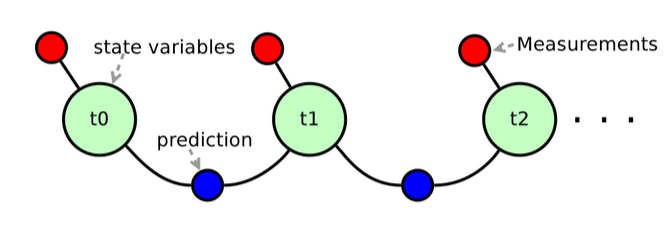
\includegraphics[width=0.7\textwidth]{factor_graph.png}
    \caption{Factor graph representation: green nodes are state variables (poses), blue nodes are motion model factors, and red nodes represent sensor measurements.}
    \label{fig:factor_graph}
\end{figure}

Mathematically, a factor graph models the joint posterior distribution over all states $X$, given observations $Z$, as a product of smaller, local functions:

\begin{equation}
P(X \mid Z) \propto \prod_k \phi_k(X_{\alpha(k)}),
\label{eq:fg_joint}
\end{equation}

where $\phi_k$ is a factor derived from a sensor model or prior, and $X_{\alpha(k)}$ is the subset of state variables relevant to that factor.

In the context of localization, let $X = \{x_0, x_1, \dots, x_n\}$ be the robot’s pose trajectory and $Z = \{z_1, \dots, z_M\}$ be the set of sensor measurements. The joint posterior can be factorized as:

\begin{equation}
P(X \mid Z) \propto P(x_0) \prod_{k=1}^n P(x_k \mid x_{k-1}) \prod_{m=1}^M P(z_m \mid X_{\alpha(m)}),
\label{eq:fg_bayes}
\end{equation}

where:
\begin{itemize}
    \item $P(x_0)$ is the prior on the initial state,
    \item $P(x_k \mid x_{k-1})$ is the motion model (e.g., from IMU preintegration),
    \item $P(z_m \mid X_{\alpha(m)})$ is the sensor measurement model (e.g., LiDAR scan matching).
\end{itemize}

Assuming Gaussian noise, the Maximum A Posteriori (MAP) estimation reduces to a nonlinear least-squares problem:

\begin{equation}
X^* = \arg\min_X \sum_k \| h_k(X_{\alpha(k)}) - z_k \|_{\Sigma_k}^2,
\label{eq:fg_map}
\end{equation}

where $h_k(\cdot)$ is the measurement function, $z_k$ is the observation, and $\Sigma_k$ is the associated noise covariance matrix.

\subsubsection{Incremental Solvers}
For real-time or large-scale applications, solving the entire problem from scratch at each step may be intractable \cite{thrun2005probabilistic}. Incremental smoothing algorithms like iSAM2 \cite{kaess2012isam2} maintain a factorization of the problem in a data structure (often a Bayes tree) that can be efficiently updated with new measurements. Rather than re-solving globally each time, iSAM2 carries out local re-linearization and partial variable reordering, providing near-constant-time updates for many practical cases.FurtherMore for Bounded computational cost , a sliding-window strategy are used to optimize only a fixed set of recent states by discarding older variables while preserving accuracy~\cite{herbert2013fusion}


\section{Research Gaps}
\label{sec:gap}
The literature review highlights several gaps and challenges in existing LiDAR-based localization systems, particularly in the context of real-time performance, scalability, and robustness. These gaps inform the design and objectives of the proposed system. Key identified gaps include:

\begin{itemize}
    \item \textbf{Long-Term Drift and Global Consistency:} Existing LIO and SLAM often suffer from long-term drift and loss of global consistency, particularly in GNSS-denied environments. While SLAM approaches attempt to address this via loop closures, their effectiveness is limited in environments with sparse or delayed loop detection.
    
    \item \textbf{Computational Intractability of MCL:} Monte Carlo Localization (MCL) is robust for 2D localization but computationally impractical for 3D due to the exponential increase in required particles. This limits its application in dense 3D point cloud and 6-DoF pose estimation.
    
    \item \textbf{Real-Time Performance and Scalability:}  map-based localization approaches struggle with real-time performance and scalability in large maps. Standard algorithms like ICP and NDT often fail to maintain real-time performance as map size increases, leading to delayed convergence or misalignment.
    
    \item \textbf{Generalization:} Existing  map-based approaches rely on handcrafted 
    features ,reflectivity profiles, or selected
    geometric structures from street-level maps limiting their generalization across diverse environments.These systems often fail to generalize across
    diverse environments and degrade in areas with low geometric richness, unmapped zones,
    or transitional boundary regions.
    
    \item \textbf{Dynamic Object Handling:} Existing systems assume static environments and do not systematically address the impact of dynamic objects on scan matching. Dynamic object removal is rarely incorporated in real-time.
    
    \item \textbf{Environmental Degradation:} Adverse conditions such as fog or sensor noise are often underrepresented in evaluation protocols, leaving a gap in understanding system resilience under realistic field conditions.
    
\end{itemize}
\cleardoublepage
point cloud\chapter{Methodology}
\label{ch:intro}

\section{System Overview}

The architecture overview and the complete step-by-step algorithm flow of the proposed localization system are shown in Figure \ref{fig:diagram-map-basedlocalization} and Algorithm \ref{alg:localization-system}. The input of the system includes the raw online point-cloud, raw IMU data as well as the prior map , and output real-time accurate 6 DOF pose.	

The system can be divided in to different modules:


\begin{enumerate}
	\item Scan Pre-Processing: Performs a series of point cloud processing steps to filter and extract relevant features from the raw LiDAR data.
	
	\item LIDAR-INERTIA Odometry - Estimates high-frequency odometry by fusing raw IMU data and LiDAR scans. The resulting odometry is added as a local constraint (odom factor) to the factor graph.
	
	\item Dynamic Local Map Loader: Generates a local map around the robot’s current pose within a specified radius from the prior map.
	
	
	\item Scan-to-Map Matching: Aligns the current LiDAR scan with the local map to estimate the robot's pose in the prior map. The estimated pose is added as a prior constraint (map factor) to the factor graph.
	
	\item Sliding Window Factor Graph Optimizer:Fuses odometry and map constraints within a sliding window to optimize and output a real-time, accurate 6-DoF pose.
	
	
\end{enumerate}

\begin{figure}
    \centering
    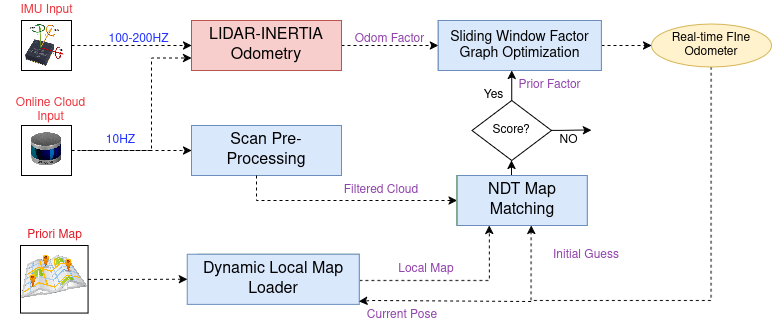
\includegraphics[width=1\linewidth]{images/system_overview.png}
    \caption{Complete Diagram of Map Based Localization}
    \label{fig:diagram-map-basedlocalization}
\end{figure}


\begin{algorithm}[H]
	\caption{LiDAR-Inertial Localization with Prior Map}
	\label{alg:localization-system}
	
	\textbf{Input:} $\mathcal{P}_t$ (LiDAR Point Cloud), $\mathcal{I}_t$ (IMU Data), $\mathcal{M}$ (Prior Map)\\
	\textbf{Output:} $\mathbf{T}_t$ (Real-time 6-DoF Pose)
	
	\begin{algorithmic}[1]
		
		\While{System is running}
		
		\State Acquire LiDAR point cloud $\mathcal{P}_t$ and IMU data $\mathcal{I}_t$
		
		\State Perform scan pre-processing on $\mathcal{P}_t$ to obtain filtered point cloud $\mathcal{P}_t^{filtered}$
		
		\State Estimate LiDAR-Inertial Odometry using $\{\mathcal{P}_t^{filtered}, \mathcal{I}_t\}$ to obtain odometry pose $\mathbf{T}_t^{lio}$	
		
		\If{$|| \mathbf{T}_t - \mathbf{T}_{last}^{map} || > d_{threshold}$}
		\State Load dynamic local map $\mathcal{M}_t^{local}$ from $\mathcal{M}$ centered at $\mathbf{T}_t^{lio}$
		\State Update $\mathbf{T}_{last}^{map} \gets \mathbf{T}_t$
		\EndIf
		
		\State Perform scan-to-map matching between $\mathcal{P}_t^{filtered}$ and $\mathcal{M}_t^{local}$ to obtain map-based pose $\mathbf{T}_t^{map}$
		
		\If{Matching score $> s_{threshold}$}
		\State Add prior factor with $\mathbf{T}_t^{map}$ to factor graph
		\EndIf
		
		\State Add odometry factor with $\mathbf{T}_t^{lio}$ to factor graph
		
		\State Optimize sliding window factor graph to obtain final pose $\mathbf{T}_t$
		
		\EndWhile
		
	\end{algorithmic}
\end{algorithm}


\subsection{LIDAR Scan Pre-Processing}
Before aligning each incoming LiDAR scan to the global map, we first subject the raw point cloud to a series of preprocessing operations. These operations improve both efficiency and reliability by filtering out irrelevant regions and outliers, downsampling to reduce data volume, and transforming the data into a consistent coordinate frame.Our approach, illustrated in Figure\ref{fig:lidar_scan_preprocessing}  consists of the following  main steps:
\begin{figure}
    \centering
    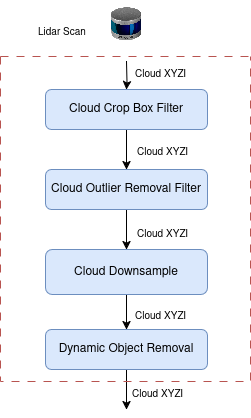
\includegraphics[width=0.4\linewidth]{images/LIDAR_PreProccess.drawio.png}
    \caption{LIDAR scan pre-processing}
    \label{fig:lidar_scan_preprocessing}
\end{figure}

\begin{itemize}
    \item \textbf{Crop-Box Filter}: This step confines the point cloud to a user-defined three-dimensional region (a bounding “box”) around the sensor or area of interest. By discarding all points lying outside this box, we focus only on the relevant portion of the scene, reducing both memory and computational overhead for subsequent processing.
    \item \textbf{Outlier Removal}: Once the point cloud is restricted to the area of interest, we remove random noise and spurious measurements using a statistical outlier filter. Concretely, we compute for each point the average distance to its k‐nearest neighbors. Points whose mean distance exceeds the global mean plus a chosen multiplier of the standard deviation are marked as outliers and deleted. This practice is a commonly adopted heuristic that discards stray or floating points, which might result from occasional sensor glitches or moving objects in the environment.
    \item \textbf{Voxel-Grid Downsampling} To further ease computational load, the point cloud is then downsampled. A typical approach uses a voxel-grid filter: space is subdivided into small volumetric “voxels,” and all points within each voxel are replaced by a single representative (often the centroid). This retains the main geometry while reducing point density, thereby speeding up map‐based matching algorithms.
    \item \textbf{Coordinate Transformation}:   Finally, we apply a rigid transformation that aligns the processed point cloud to a consistent coordinate frame used throughout our localization pipeline—the vehicle’s base link frame.This accounts for any known extrinsic offsets between the LiDAR sensor and the vehicle origin.
\end{itemize}

As summarized in Table~\ref{tab:lidar_preprocessing}, the LiDAR preprocessing parameters vary depending on the sensor type and application requirements. All filtering and scan processing operations are implemented using the Point Cloud Library (PCL).



\begin{table}[htbp]
\centering
\caption{LiDAR Scan Processing Methods and Parametrs  Across Different Sensor Setups}
\label{tab:lidar_preprocessing}
\begin{tabular}{|p{3.5cm}|p{3.5cm}|p{3.5cm}|p{3.5cm}|}
\hline
\textbf{Processing Step} & \textbf{KITTI(Velodyne HDL-64E)} & \textbf{MulRan(Ouster-OS1-64)} & \textbf{(Ouster-OS1-128)} \\
\hline
LiDAR Type & Velodyne HDL-64E & Ouster OS1-64 & Ouster OS1-128 \\
% \hline
% \textbf{Vertical Channels} & 64 & 64 & 128 \\
% \hline
% \textbf{Vertical FOV} & $\pm$2° to $\pm$24.8° ($\sim$26.8° total) & $\pm$16.6° ($\sim$33.2° total) & $\pm$22.5° ($\sim$45° total) \\
\hline
Max Range & $\sim$120 m & $\sim$120 m & $\sim$240 m \\
\hline
Crop Box Filter & 90-100m & 90-100m & 180-200m\\
\hline
Downsampling Method & Voxel-Grid(leaf-size: 0.5m) & Voxel-Grid(leaf-size: 0.4-0.6 m) & Voxel-Voxel(0.5-0.8 m) \\
\hline
Outlier Removal & Statistical (K=50, Std=1.0) & Statistical (K=40, Std=1.0) & Statistical(K=40 ,Std=1,0) \\
\hline
% \textbf{Ground Removal} & Not used & Yes — flat surface segmentation &  Yes — flat surface segmentation \\
% \hline
\end{tabular}
\end{table}

\subsection{Map Pre-Processing}

\subsubsection{Grid-based Map Point Cloud Division }

When using a high-resolution point cloud map for localization in large areas, loading the entire map can overwhelm memory and computation. To tackle this, \emph{we divide the global map} into smaller ``tiles,'' each containing only part of the overall data as shown in \ref{fig:pointcloud division}. Below is a brief outline:

\begin{itemize}
    \item \textbf{Rationale}: Instead of loading the entire map, the localization system can dynamically fetch only the sub-map (tile) around the vehicle's estimated position, saving memory and speeding up matching.
    \item \textbf{Grid Definition}: A user-chosen tile size (e.g., 100\,m\,$\times$\,100\,m) defines a regular grid overlay on the map's bounding box. Each tile's data are saved as a separate file.
    \item \textbf{Offline Preparation}: This division happens once, offline. The resulting sub-map files (e.g., \texttt{tile\_0\_0.pcd}, \texttt{tile\_1\_0.pcd}) are stored on disk.
    \item \textbf{Tile Indexing}: A simple coordinate scheme (e.g., $(i, j)$ for each tile) allows quick lookup. As the vehicle moves, the system checks its approximate position and loads only the necessary tiles.
\end{itemize}

\begin{figure}
    \centering
    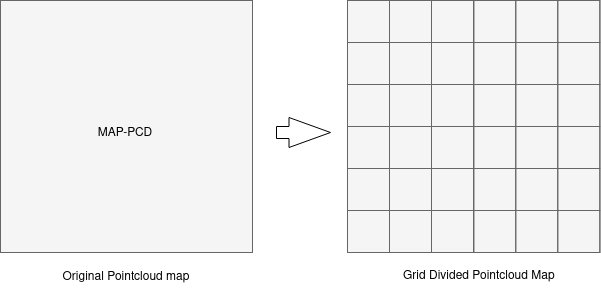
\includegraphics[width=0.8
    \linewidth]{images/map.drawio.png}
    \caption{Grid Based Point-cloud division }
    \label{fig:pointcloud division}
\end{figure}
\subsection{Dynamic Map Loading}

Even with a divided map, loading all tiles at once is inefficient. Therefore, the system adopts a \emph{dynamic loading} strategy, where only the sub-clouds near the robot's current position are fetched in real time. Concretely:

\begin{itemize}
    \item \textbf{Robot Pose Check}: At each iteration (or after the robot travels a threshold distance), the system retrieves the robot's latest pose estimate.
    \item \textbf{Loading Radius}: Based on sensor range (e.g., LiDAR maximum range) and a user-defined margin, we determine a radius (e.g., 80\,m) around the current pose within which map data is required.
    \item \textbf{Partial Tile Retrieval}: Only tiles intersecting this radius are loaded, reducing memory overhead. As the robot moves and crosses tile boundaries, newly relevant tiles are loaded and old ones are freed.
    \item \textbf{Update Frequency}: To avoid frequent reloads, the system triggers map updates only after the robot has moved a certain threshold (e.g., 20\,m) since the last update.
\end{itemize}

This on-demand \emph{dynamic loading} ensures that the system retains sufficient map detail for accurate localization while minimizing both I/O and memory consumption. 

\subsection{LIDAR Inertia Odometry}

\subsection{Scan-to-Map Matching}

\subsubsection{}






\cleardoublepage
%\chapter{Result}
\label{ch:intro}

\section{Experimental Environment}

\subsection{Hardware Setup}
All experiments were conducted on a development laptop equipped with an AMD Ryzen™ 7 7735HS processor, 32 GB of DDR5 RAM, and an NVIDIA GPU for accelerated computation , as well as on a \emph{Hunter} mobile robotic platform for on-campus data collection.The robot is equipped with a suite of sensors, including a 3D LiDAR sensor for environment perception, an Inertial Measurement Unit (IMU) for estimating motion and orientation, and a camera for visual reference. An onboard NVIDIA CPU/GPU computing module provides local processing capability.

\begin{figure}[H]
	\centering
	\begin{minipage}{0.5\textwidth}
		\centering
		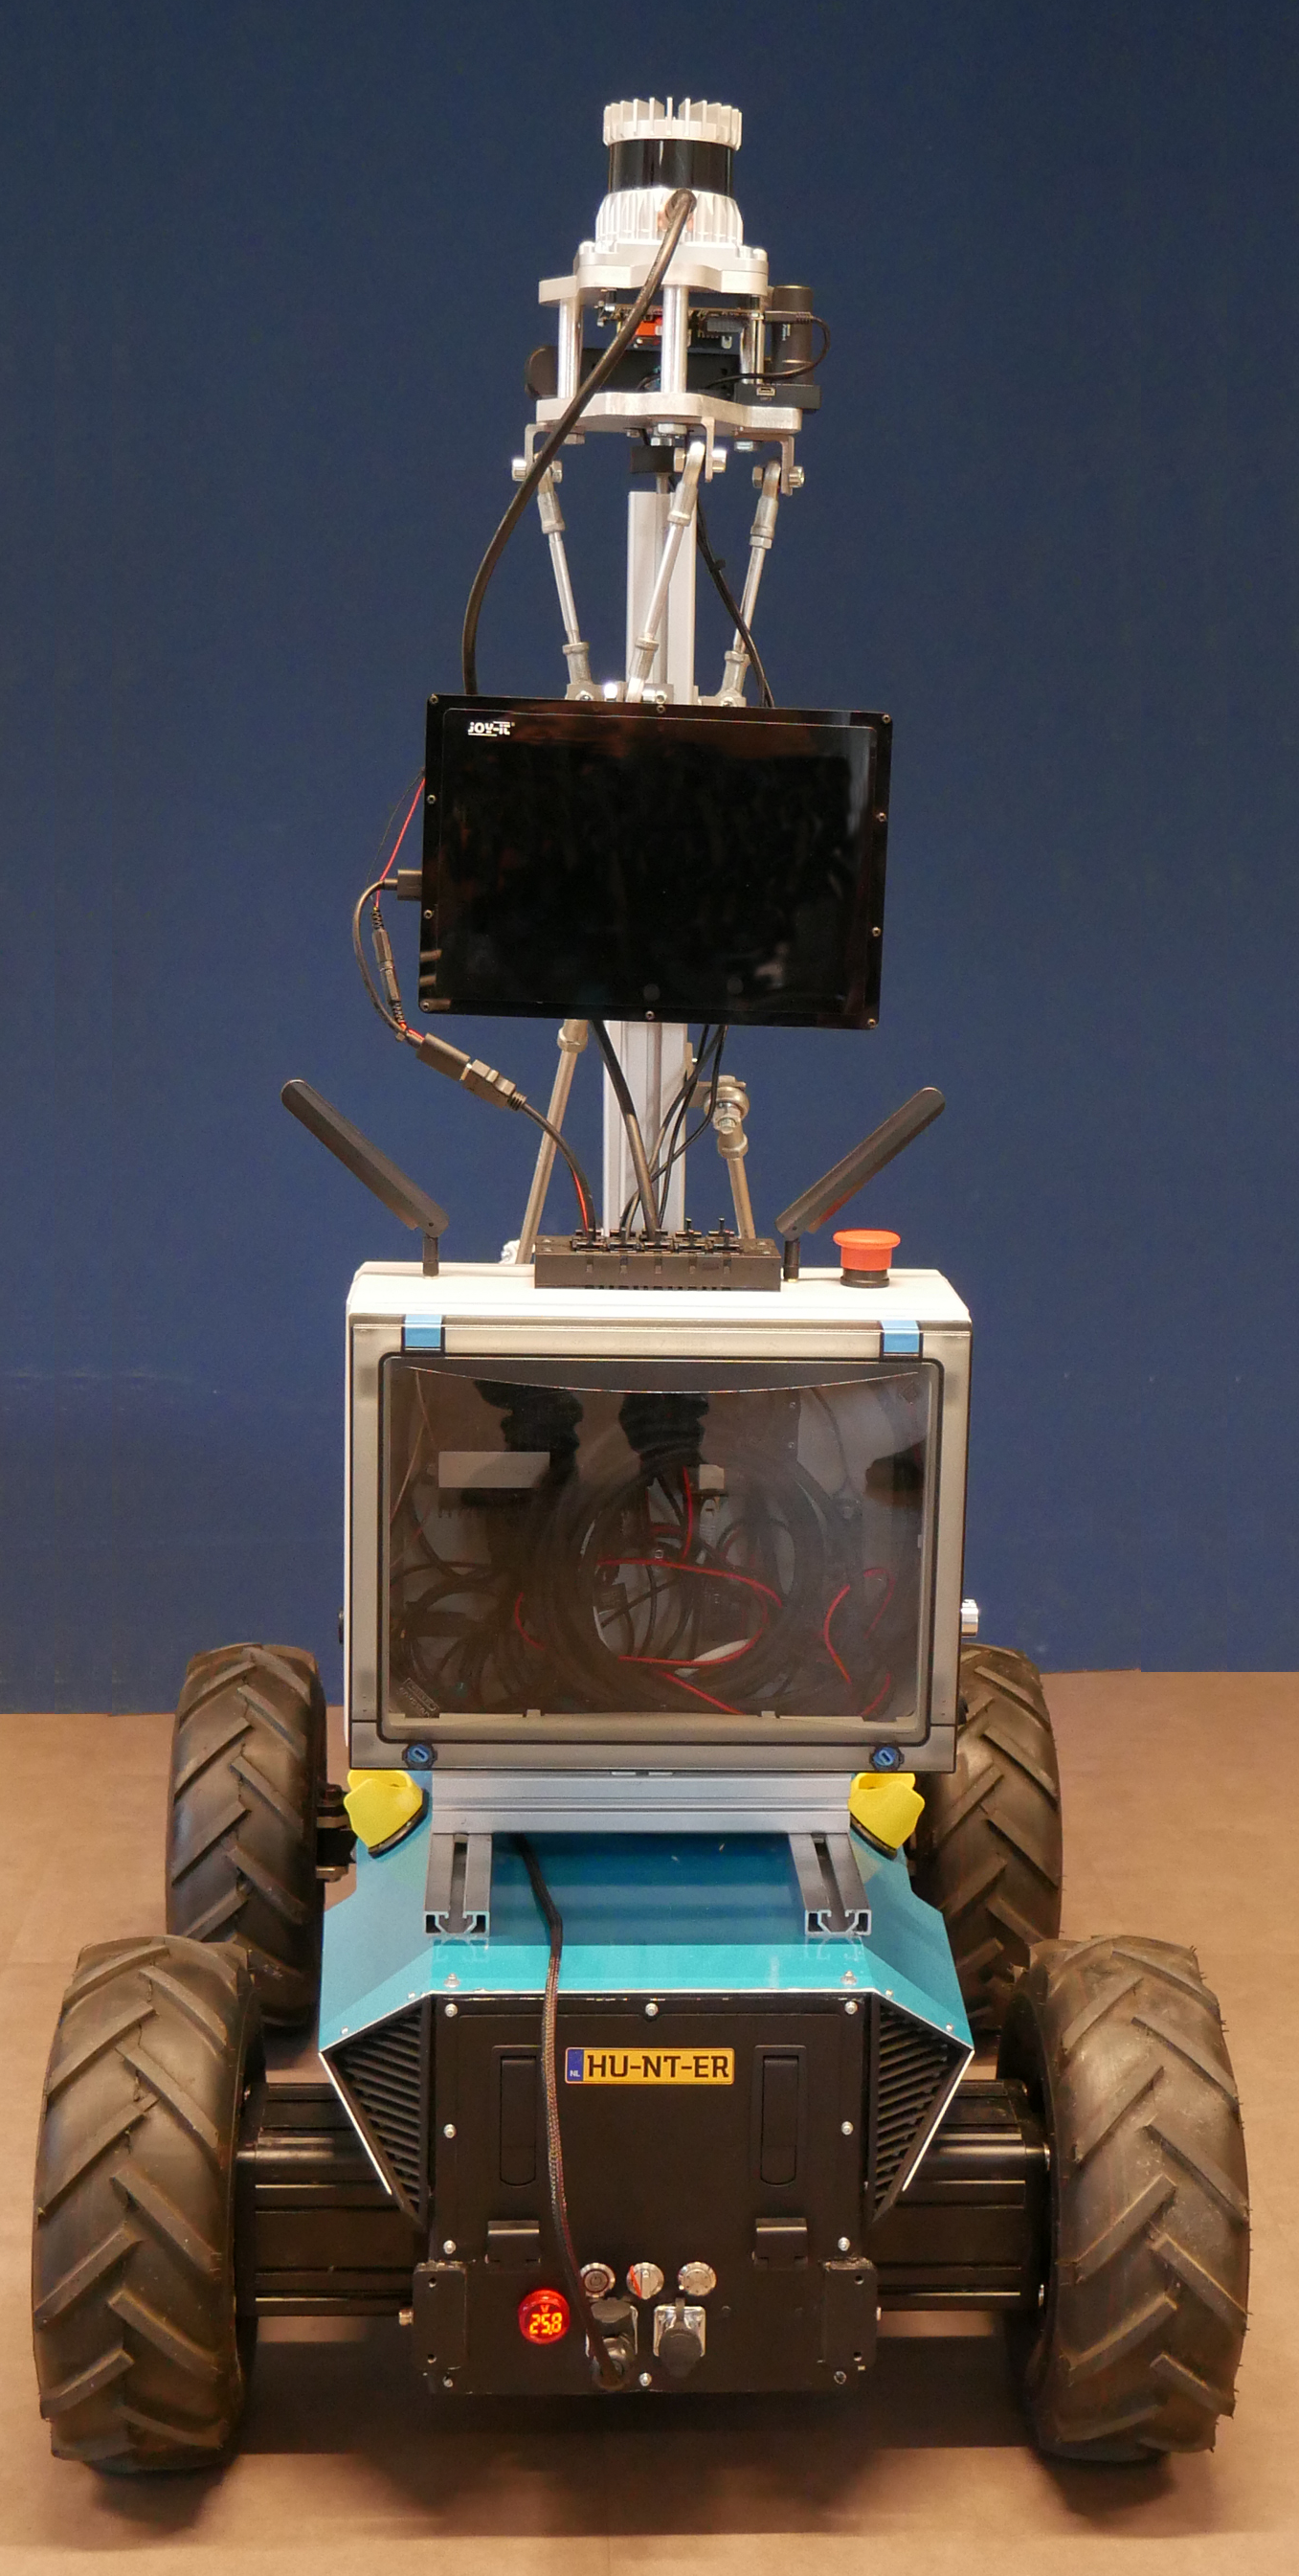
\includegraphics[height=6cm , width=4cm]{images/Hunter_body.png}
		\caption*{(a) Hunter mobile robot platform}
	\end{minipage}\hfill
	\begin{minipage}{0.5\textwidth}
		\centering
		\includegraphics[height=6cm , width=4cm]{images/Hunter_sensor.png}
		\caption*{(b) Sensor configuration (LiDAR, IMU, Camera)}
	\end{minipage}
	\caption{Hardware setup used for real-world data collection and testing: (a) Hunter robotic platform; (b) onboard sensors.}
	\label{fig:hunter-robot-setup}
\end{figure}


\subsection{Software Setup}
Our approach is implemented primarily in C++ on top of the ROS\,2 Humble middleware. We rely on:
\begin{itemize}
  \item \textbf{PCL (Point Cloud Library):} for point cloud data structures and filtering.
  \item \textbf{Eigen:} for linear algebra operations (transformations, matrix computations).
  \item \textbf{ROS\,2 Bag Files:} each dataset is provided or recorded in a \texttt{.bag} format, facilitating playback of sensor data.
\end{itemize}
Additional scripts in Python were employed for plotting and minor data manipulations.

\subsection{Datasets}
We evaluated our map-based localization on multiple datasets, each of which offers LiDAR and IMU data. Table~\ref{tab:datasets} summarizes their key characteristics.

\begin{table}[htbp]
	\centering
	\caption{Overview of datasets and sensor configurations. (L: LiDAR; I: IMU)}
	\label{tab:datasets}
	\resizebox{\textwidth}{!}{%
	\begin{tabular}{lccccc}
	\toprule
	\textbf{Dataset} & \textbf{Seq.} & \textbf{Sensors} & \textbf{LiDAR Type} & \textbf{Frequencies (Hz)} & \textbf{Map Prep. Method} \\
	\midrule
	\textbf{KITTI Odometry} & 05 & L + I & Velodyne HDL-64E & L: 10, I: 100 & GT-based aggregation \\
	%\textbf{KITTI Odometry} & 09 & L + I & Velodyne HDL-64E & L: 10, I: 100 & GT-based aggregation \\
	\textbf{MulRan}         & KiAST-02,03 & L + I & Ouster OS1-64    & L: 10, I: 100 & Fast-LIO2 SLAM \\
	\textbf{Saxion campus}  & seq1,2,3 & L + I & Ouster OS1-128    & L: 10, I: 100 & Fast-LIO2 SLAM \\
	
	\bottomrule
	\end{tabular}%
	}
\end{table}

\paragraph{KITTI Sequences}
We tested on sequences 05 from the KITTI odometry benchmark\cite{Geiger2012KITTI}. These sequences contain semi-urban driving scenarios with moderate speeds. Each frame is timestamped and stored in a ROS\,2 bag for convenient playback.

\paragraph{MulRan (KiAST) Sequences}
Two sequences (KiAST-02, KiAST-03) from the MulRan dataset\cite{Kim2020Mulran} were used. These contain Ouster OS1-64 LiDAR and IMU measurements in campus-like settings with dynamic objects and complex geometry. The ROS\,2 bags allow consistent replay for algorithm testing.

\subsection{Map Preparation}
For each dataset, a prior 3D map was generated before running the localization:

\begin{itemize}
    \item \textbf{KITTI:} We leveraged the official ground-truth poses to transform and aggregate each LiDAR frame into a global coordinate system. The resulting dense point cloud was lightly downsampled (e.g., voxel size of 0.1\,m).
    \item \textbf{MulRan (KAiST) and Campus (Saxion) Dataset:} No direct ground truth was provided, so we employed \textit{Fast-LIO2 SLAM} to build a consistent map from repeated traversals. This method fuses LiDAR scans and IMU data for robust odometry. The final aggregated map was also voxel-downsampled.
\end{itemize}

In both cases, the final global point cloud is subdivided into manageable tiles for efficient dynamic loading during localization. Each tile is stored as a separate file or database entry keyed by tile coordinates, allowing the system to load only relevant tiles based on the vehicle’s current estimated position.



\section{Performance Evaluation}
This section presents the experimental results evaluating the proposed LiDAR-inertial localization system. The evaluation is divided into two main parts: performance under standard conditions, and extended experiments conducted under different scenarios to assess system robustness. Standard conditions refer to scenario where the reference map is up-to-date, sensor data is relatively noise-free, and feature-rich map. In contrast, under extended scenarios, we test robustness by replaying the same trajectory through map transition zones, with composite geometric noise (simulating fog, rain, and snow), slight map aging, and dynamic object removal.Overall,we evaluate localization performance in terms of Absolute Pose Error, convergence behavior, and real-time processing latency.

Overall, we evaluate localization performance in terms of Absolute Pose Error (APE), convergence behavior, and real-time processing latency. The evaluation includes comparisons against two categories of baselines: component baselines, which consist of the individual modules integrated into our system (Fast-LIO2\cite{xuFastLIO2} and NDT\cite{biber2003ndt} scan matching), and external SLAM baselines, such as MOLA\cite{blanco2025mola_lo} and KISS-ICP\cite{kiss2025arxiv}, which represent complete state estimation frameworks used for comparative benchmarking.

\subsection{ Localization Performance in Standard Conditions}

\subsubsection{Saxion Campus Dataset}
We evaluated our proposed LiDAR-inertial localization system on three sequences collected from the Saxion campus, representing short, medium, and long trajectories with varying coverage areas and trajectory complexity.Quantitative performance is assessed using Absolute Pose Error (APE) and rotational error after SE(3) alignment.

 Table \ref{tab:ape_rot_saxion_seq1} , \ref{tab:ape_rot_saxion_seq2} , \ref{tab:ape_rot_saxion_seq3} summarize translation and rotation error statistics, including maximum, mean, and RMSE values for the three Saxion sequences. The results show that the proposed fusion-based system consistently outperforms both baseline methods across all sequences. In Sequence 1, the proposed method achieves centimeter-level accuracy, with  translation RMSE of 0.067 m, which is approximately 33× lower than the RMSE of 2.197 m observed with Fast-LIO2. The rotational RMSE is also reduced from 2.072° to 0.583°, indicating significant drift correction not only in position but also in orientation.

 In the longer and more complex trajectories (Sequences 2 and 3), the proposed fusion method achieves decimeter-level accuracy, significantly reducing translational RMSE compared to Fast-LIO2 (from 3.3 m to 0.11–0.13 m) and improving rotational RMSE by up to 1.6°. While NDT achieves similar translational RMSE in some cases, the fusion method offers better rotational accuracy and stability, especially under challenging conditions.
 
Trajectory plots Figures \ref{fig:saxion-seq1-trajectory-zoom}~ \ref{fig:saxion-seq2-trajectory-zoom}~\ref{fig:saxion-seq3-trajectory-zoom}  illustrate the alignment of estimated poses with reference trajectory. Zoomed-in regions further emphasize the proposed method’s ability to track the trajectory accurately, even in complex zones and long trajectory.Overall, these results confirm that the proposed system provides robust and drift-resilient localization across short, medium, and long trajectories, maintaining centimeter- to decimeter-level precision under varying compexity.



\begin{table}[H]
	\centering
	\renewcommand{\arraystretch}{0.6}
	\setlength{\tabcolsep}{15pt}
	\caption{Translation (APE) and Rotation Error statistics for Saxion \textbf{Sequence 1} }
	\captionsetup{justification=justified, singlelinecheck=false}
	
	
	\label{tab:ape_rot_saxion_seq1}
	
	\begin{adjustbox}{width=\textwidth}
		\begin{tabular}{@{}lccccccc@{}}
			\toprule
			\textbf{Method} & \textbf{Metric} & \textbf{Max} & \textbf{Mean} & \textbf{Median} & \textbf{Min} & \textbf{RMSE} & \textbf{Std Dev} \\
			\midrule
			
			\multirow{2}{*}{\textbf{Proposed (Fusion)}} 
			& APE (m)        & 0.395   & \textbf{0.052 }   & \textbf{0.041}     & \textbf{0.003 }   &\textbf{ 0.067}   & \textbf{0.042 }\\
			& Rot. (deg)     & \textbf{4.715}   & \textbf{0.321}    & \textbf{0.169}     &\textbf{ 0.030 }   & \textbf{0.583}   &\textbf{ 0.486} \\
			\midrule
			
			\multirow{2}{*}{NDT Scan Matching} 
			& APE (m)        & \textbf{0.363 }  & 0.074    & 0.067     & 0.012    & 0.084   & \textbf{0.041} \\
			& Rot. (deg)     & 5.832   & 0.503    & 0.299     &\textbf{ 0.012}    & 0.813   & 0.639 \\
			\midrule
			
			\multirow{2}{*}{Fast-LIO2} 
			& APE (m)        & 7.594   & 1.456    & 0.933     & 0.322    & 2.197   & 1.645 \\
			& Rot. (deg)     & 6.213   & 1.631    & 1.304     & 0.419    & 2.072   & 1.278 \\
			\bottomrule
		\end{tabular}
	\end{adjustbox}
\vspace{0.5em}
{\footnotesize \textit{Note:} Bold values indicate the best performance across each metric.}
\end{table}

\begin{figure}[H]
	\centering
	\begin{tikzpicture}
		% Main trajectory image
		\node[anchor=south west, inner sep=0] (main) at (0,0)
		{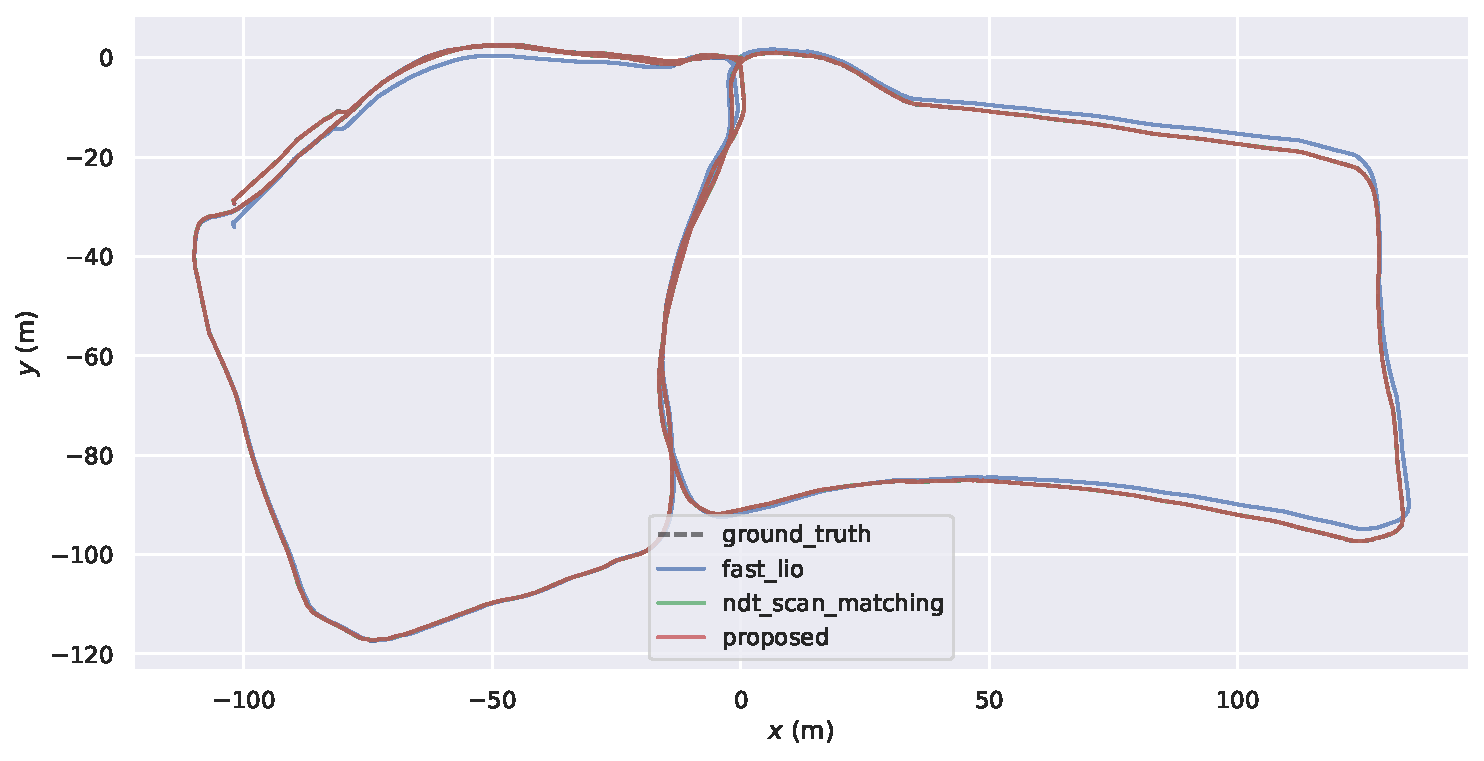
\includegraphics[page=1 , width=0.8\textwidth]{images/trajectory_plot_seq1.pdf}};
		% Coordinate system normalized to the image
		\begin{scope}[x={(main.south east)}, y={(main.north west)}]
			% Red dashed rectangle for zoom box (adjust coordinates!)
			\draw[red, thick, dashed] (0.85, 0.20) rectangle (0.98, 0.45);
			% Red arrow from zoom box to zoomed-in image
			\draw[->, red, thick] (0.98, 0.45) -- (1, 0.85);
		\end{scope}
		% Zoomed-in image overlay (use exact x/y in cm to place)
		\node[anchor=south west] at (8, 6)
		{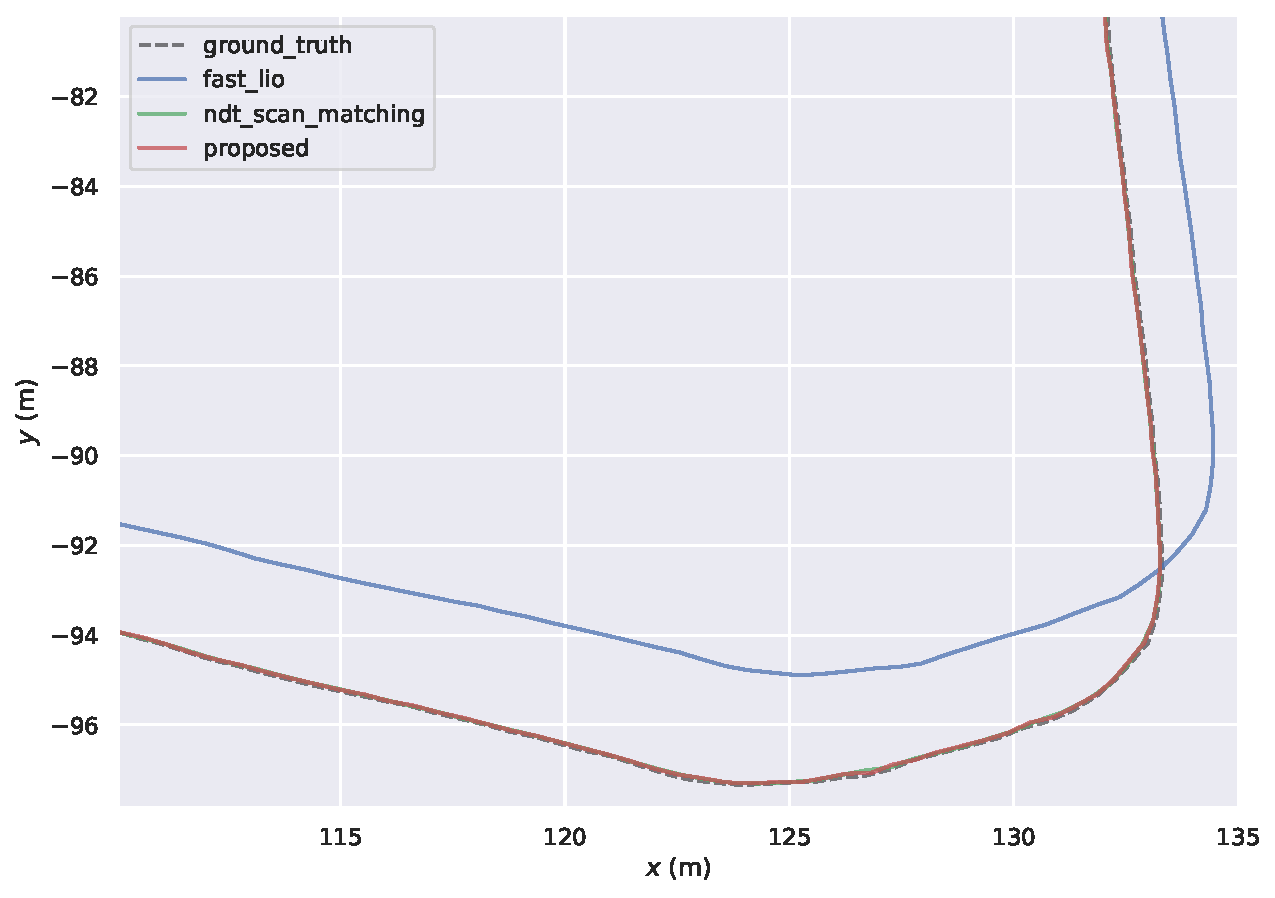
\includegraphics[width=0.5\textwidth]{images/trajectory_zoom_seq1.pdf}};
		% Optional label
		%\node at (15, 4.6) {\small Zoomed-in detail};
	\end{tikzpicture}
	\caption[Saxion Sequence 01 – Trajectory Alignment with Zoomed Comparison]%
	{\textbf{Saxion Sequence 01 – Trajectory Alignment.} 
		The figure shows the estimated trajectories from FAST-LIO2, low frequency NDT map matching , and the proposed method, overlaid against ground truth. The red dashed box indicates the zoomed region.
	}
	\label{fig:saxion-seq1-trajectory-zoom}
\end{figure}


\begin{table}[H]
	\centering
	\renewcommand{\arraystretch}{0.6}
	\setlength{\tabcolsep}{15pt}
	\caption{Translation (APE) and Rotation Error statistics for Saxion \textbf{Sequence 2} }
	\label{tab:ape_rot_saxion_seq2}
	
	\begin{adjustbox}{width=\textwidth}
		\begin{tabular}{@{}lccccccc@{}}
			\toprule
			\textbf{Method} & \textbf{Metric} & \textbf{Max} & \textbf{Mean} & \textbf{Median} & \textbf{Min} & \textbf{RMSE} & \textbf{Std Dev} \\
			\midrule
			
			\multirow{2}{*}{\textbf{Proposed (Fusion)}} 
			& APE (m)        & 0.440   & \textbf{0.090}   & \textbf{0.075}     & \textbf{0.005}   & \textbf{0.107}   & \textbf{0.058} \\
			& Rot. (deg)     & 4.356   & \textbf{0.782}   & \textbf{0.539}     & \textbf{0.051}   & \textbf{1.046}   & \textbf{0.695} \\
			\midrule
			
			\multirow{2}{*}{NDT Scan Matching} 
			& APE (m)        & \textbf{0.245}   & 0.102   & 0.094     & 0.009    & 0.118   & 0.059 \\
			& Rot. (deg)     & \textbf{2.639}   & 1.195   & 1.127     & 0.103    & 1.393   & 0.715 \\
			\midrule
			
			\multirow{2}{*}{Fast-LIO2} 
			& APE (m)        & 9.467   & 2.507   & 1.944     & 0.370    & 3.301   & 2.147 \\
			& Rot. (deg)     & 5.494   & 2.250   & 1.568     & 0.202    & 2.680   & 1.456 \\
			\bottomrule
		\end{tabular}
	\end{adjustbox}

\vspace{0.5em}
{\footnotesize \textit{Note:} Bold values indicate the best performance across each metric.}
\end{table}


\begin{table}[H]
	\centering
	\renewcommand{\arraystretch}{0.6}
	\setlength{\tabcolsep}{15pt}
	\caption{Translation (APE) and Rotation Error statistics for Saxion \textbf{Sequence 3} }
	\label{tab:ape_rot_saxion_seq3}
	
	\begin{adjustbox}{width=\textwidth}
		\begin{tabular}{@{}lccccccc@{}}
			\toprule
			\textbf{Method} & \textbf{Metric} & \textbf{Max} & \textbf{Mean} & \textbf{Median} & \textbf{Min} & \textbf{RMSE} & \textbf{Std Dev} \\
			\midrule
			
			\multirow{2}{*}{\textbf{Proposed (Fusion)}} 
			& APE (m)        & 0.821   & \textbf{0.097}   & \textbf{0.072}     & \textbf{0.004}   & 0.135   & 0.094 \\
			& Rot. (deg)     & 5.016   & \textbf{0.725}   & \textbf{0.472}     & \textbf{0.076}   & \textbf{1.039}   & \textbf{0.743} \\
			\midrule
			
			\multirow{2}{*}{NDT Scan Matching} 
			& APE (m)        & \textbf{0.297}   & 0.113   & 0.100     & 0.025    & \textbf{0.126}   & \textbf{0.056} \\
			& Rot. (deg)     & 3.236   & 1.373   & 1.286     & 0.131    & 1.652   & 0.919 \\
			\midrule
			
			\multirow{2}{*}{Fast-LIO2} 
			& APE (m)        & 3.475   & 1.468   & 1.254     & 0.028    & 1.862   & 1.145 \\
			& Rot. (deg)     & 2.750   & 0.955   & 0.953     & 0.069    & 1.088   & 0.522 \\
			\bottomrule
		\end{tabular}
	\end{adjustbox}
{\footnotesize \textit{Note:} Bold values indicate the best performance across each metric.}
\end{table}



\subsubsection{Comparison with SLAM Methods }

To benchmark the proposed system against existing SLAM methods, we evaluated it on KITTI Sequence 05, which includes multiple natural loop closures alongside KISS-ICP  and MOLA SLAM. As shown in Table~\ref{tab:ape_rot_kitti_seq5}, the proposed method achieves significantly lower translation and rotation errors, attaining decimeter-level accuracy through the incorporation of map-based scan matching and factor-graph fusion.

Despite the presence of loop closures, both SLAM methods exhibit notable drift and large maximum errors with translational APE reaching up to 6.8\,m and rotational errors exceeding {3.8°}. These results underline a key limitation of SLAM: its reliance on successful and timely loop closure events to correct long-term drift. In contrast, the proposed approach leverages a prebuilt map to maintain global consistency at all times, avoiding error accumulation. As visualized in Figure~\ref{fig:kitti05-traj-zoom}, the proposed trajectory remains well-aligned with the reference path throughout the sequence, while SLAM methods show clear deviation, especially toward the end. This demonstrates the robustness and reliability of map-based localization  even under conditions favorable to SLAM.

\begin{table}[H]
	\centering
	\renewcommand{\arraystretch}{0.6}
	\setlength{\tabcolsep}{15pt}
	\caption{Translation (APE) and Rotation Error statistics for \textbf{KITTI Sequence 05}}
	\label{tab:ape_rot_kitti_seq5}
	
	\begin{adjustbox}{width=\textwidth}
		\begin{tabular}{@{}lccccccc@{}}
			\toprule
			\textbf{Method} & \textbf{Metric} & \textbf{Max} & \textbf{Mean} & \textbf{Median} & \textbf{Min} & \textbf{RMSE} & \textbf{Std Dev} \\
			\midrule
			
			\multirow{2}{*}{\textbf{Proposed}} 
			& APE (m)        & \textbf{0.483}   & \textbf{0.121}   & \textbf{0.102}     & \textbf{0.007}   & \textbf{0.143}   & \textbf{0.077} \\
			& Rot. (deg)     & \textbf{1.914}   & \textbf{0.376}   & \textbf{0.356}     & \textbf{0.078}   & \textbf{0.402}   & \textbf{0.144} \\
			\midrule
			
			\multirow{2}{*}{KISS-ICP} 
			& APE (m)        & 5.067   & 1.460   & 1.445     & 0.281    & 1.604   & 0.666 \\
			& Rot. (deg)     & 2.696   & 1.376   & 1.441     & 0.000    & 1.465   & 0.504 \\
			\midrule
			
			\multirow{2}{*}{MOLA SLAM} 
			& APE (m)        & 6.817   & 1.539   & 1.447     & 0.306    & 1.793   & 0.920 \\
			& Rot. (deg)     & 3.861   & 1.931   & 1.886     & 0.000    & 2.015   & 0.577 \\
			\bottomrule
		\end{tabular}
	\end{adjustbox}

{\footnotesize \textit{Note:} Bold values indicate the best performance across each metric.}
\end{table}


\begin{figure}[H]
	\centering
	\begin{tikzpicture}
		
		% Main trajectory image
		\node[anchor=south west, inner sep=0] (main) at (0,0)
		{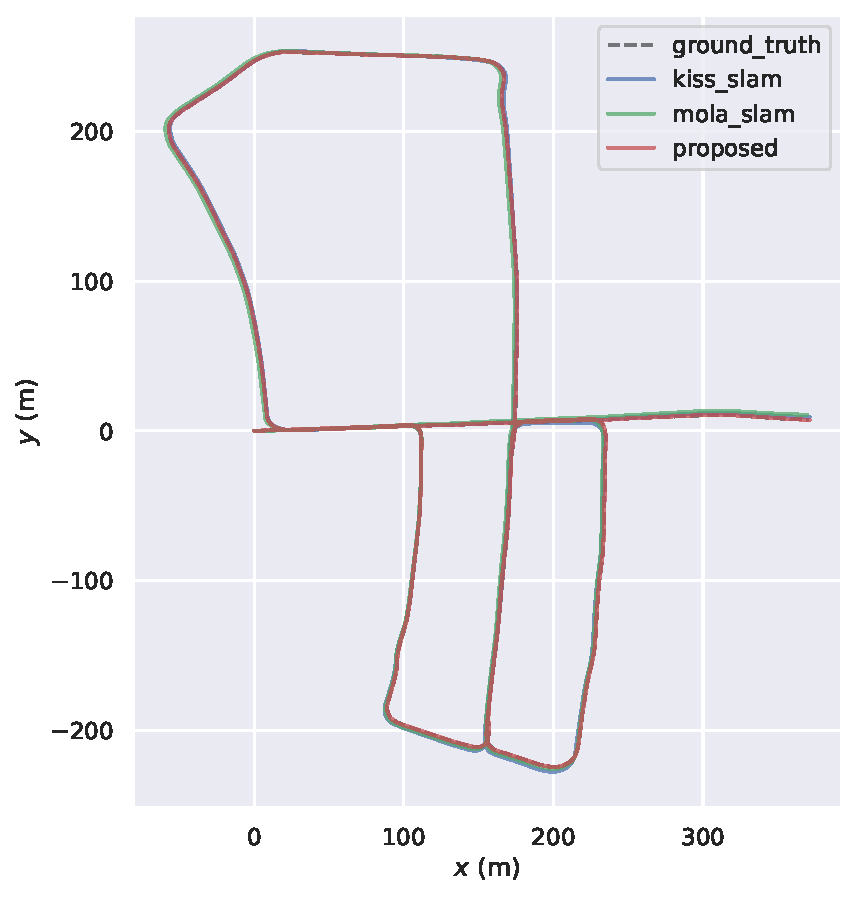
\includegraphics[width=0.75\textwidth]{images/trajectory_plot_kitti.pdf}};
		% Coordinate system normalized to the image
		\begin{scope}[x={(main.south east)}, y={(main.north west)}]
			% Red dashed rectangle for zoom box (adjust coordinates!)
			\draw[red, thick, dashed] (0.85, 0.5) rectangle (0.95, 0.56);
			% Red arrow from zoom box o tzoomed-in image
			\draw[->, red, thick] (0.95, 0.55) -- (0.97, 0.57);
		\end{scope}
		
		% Zoomed-in image overlay (use exact x/y in cm to place)
		\node[anchor=south west] at (8.1, 7.2)
		{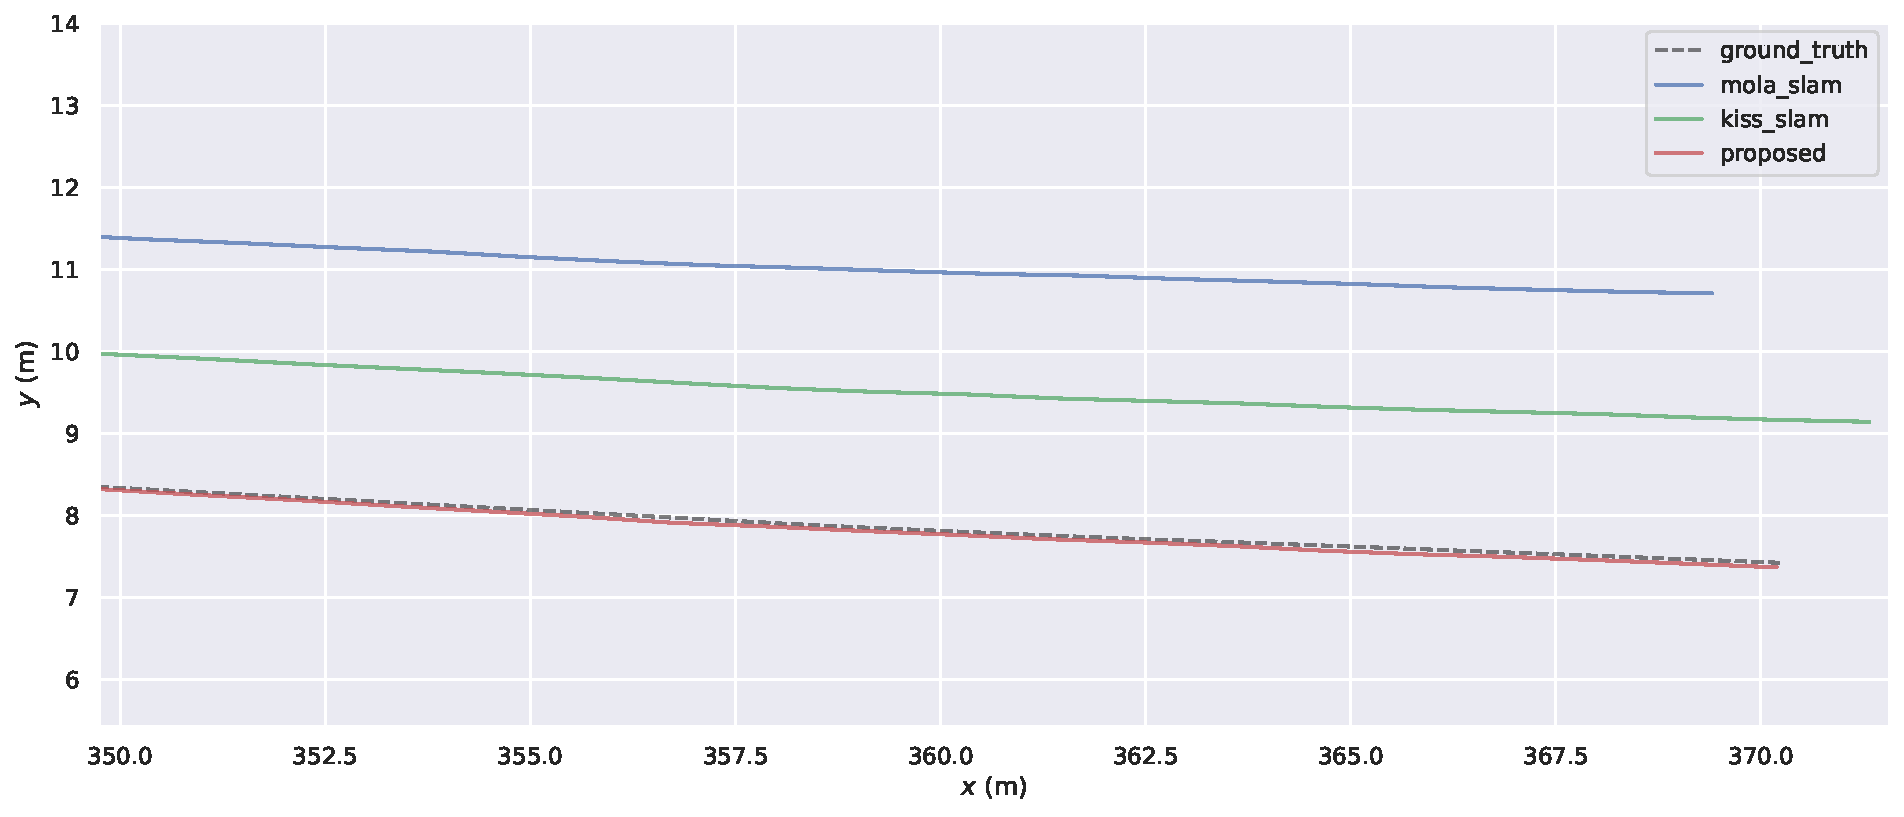
\includegraphics[width=0.45\textwidth]{images/trajectory_plot_kitti_zoom.pdf}};
		
		% Optional label
		%\node at (15, 4.6) {\small Zoomed-in detail};
		
	\end{tikzpicture}
	
	\caption[KITTI Sequence 05 – Trajectory Alignment with Zoomed Comparison]%
	{\textbf{KITTI Sequence 05 – Trajectory Alignment.} 
		The figure shows the estimated trajectories from KISS-SLAM, MOLA SLAM, and the proposed method, overlaid against ground truth.The red dashed box indicates the zoomed region..
	}
	\label{fig:kitti05-traj-zoom}
\end{figure}

\subsubsection{Real-time Performance }



We evaluate  scan-to-map matching by varying the radius of the local sub map and compare multi-threaded
NDT (NDT-OMP) , standard NDT and classic ICP all operating on identically generated local maps.As shown in the table \ref{tab:scanmap_radius} While both NDT and ICP maintain convergence on small radii (> 100 m), their per‐scan runtime  is exceed 100 ms and increases as map grows.In contrast, NDT-OMP maintains sub-25 ms mean latency with over 95 $\%$ convergence up to 200 m, and still achieves under 33 ms runtimes and 90 $\%$ convergence at 350 m (with occasional failures). This demonstrates that NDT-OMP’s parallelization, coupled with an adaptive local-map radius based on the robot’s pose, significantly improves scan-matching efficiency without sacrificing robustness.



\begin{table}[H]
	\centering
	\caption{Scan‐Matching Performance vs.\ Local Map Radius}
	\renewcommand{\arraystretch}{0.5}
	\setlength{\tabcolsep}{1pt}
	\label{tab:scanmap_radius}
	\begin{tabular}{c l c c c}
		\toprule
		\textbf{Map Radius(m)} & \textbf{Method} & \textbf{Mean Time(ms)} & \textbf{Converged(\%)} & \textbf{Remarks} \\
		\midrule
		100 & NDT     & 90  & 90 &  \\
		& ICP     & >100  & 90 &             \\
		& NDT‐OMP(8 thread) &  15  & 99 &     \\
			\midrule
		\addlinespace
		200 & NDT     & >100  & <50 &  failures           \\
		& ICP     & >100  & <50&       failures     \\
		& NDT‐OMP(8 thread) & 20  & 97 &            \\
			\midrule
		\addlinespace
		350 & NDT     & >100  & <50 &  failures \\
		& ICP     & >100 &     <50 &  failures          \\
		& NDT‐OMP(8 thread) & 25  & 90 &  some failures     \\
		\bottomrule
	\end{tabular}
\end{table}

\begin{figure}[H]
	\centering
	\begin{subfigure}[t]{0.48\textwidth}
		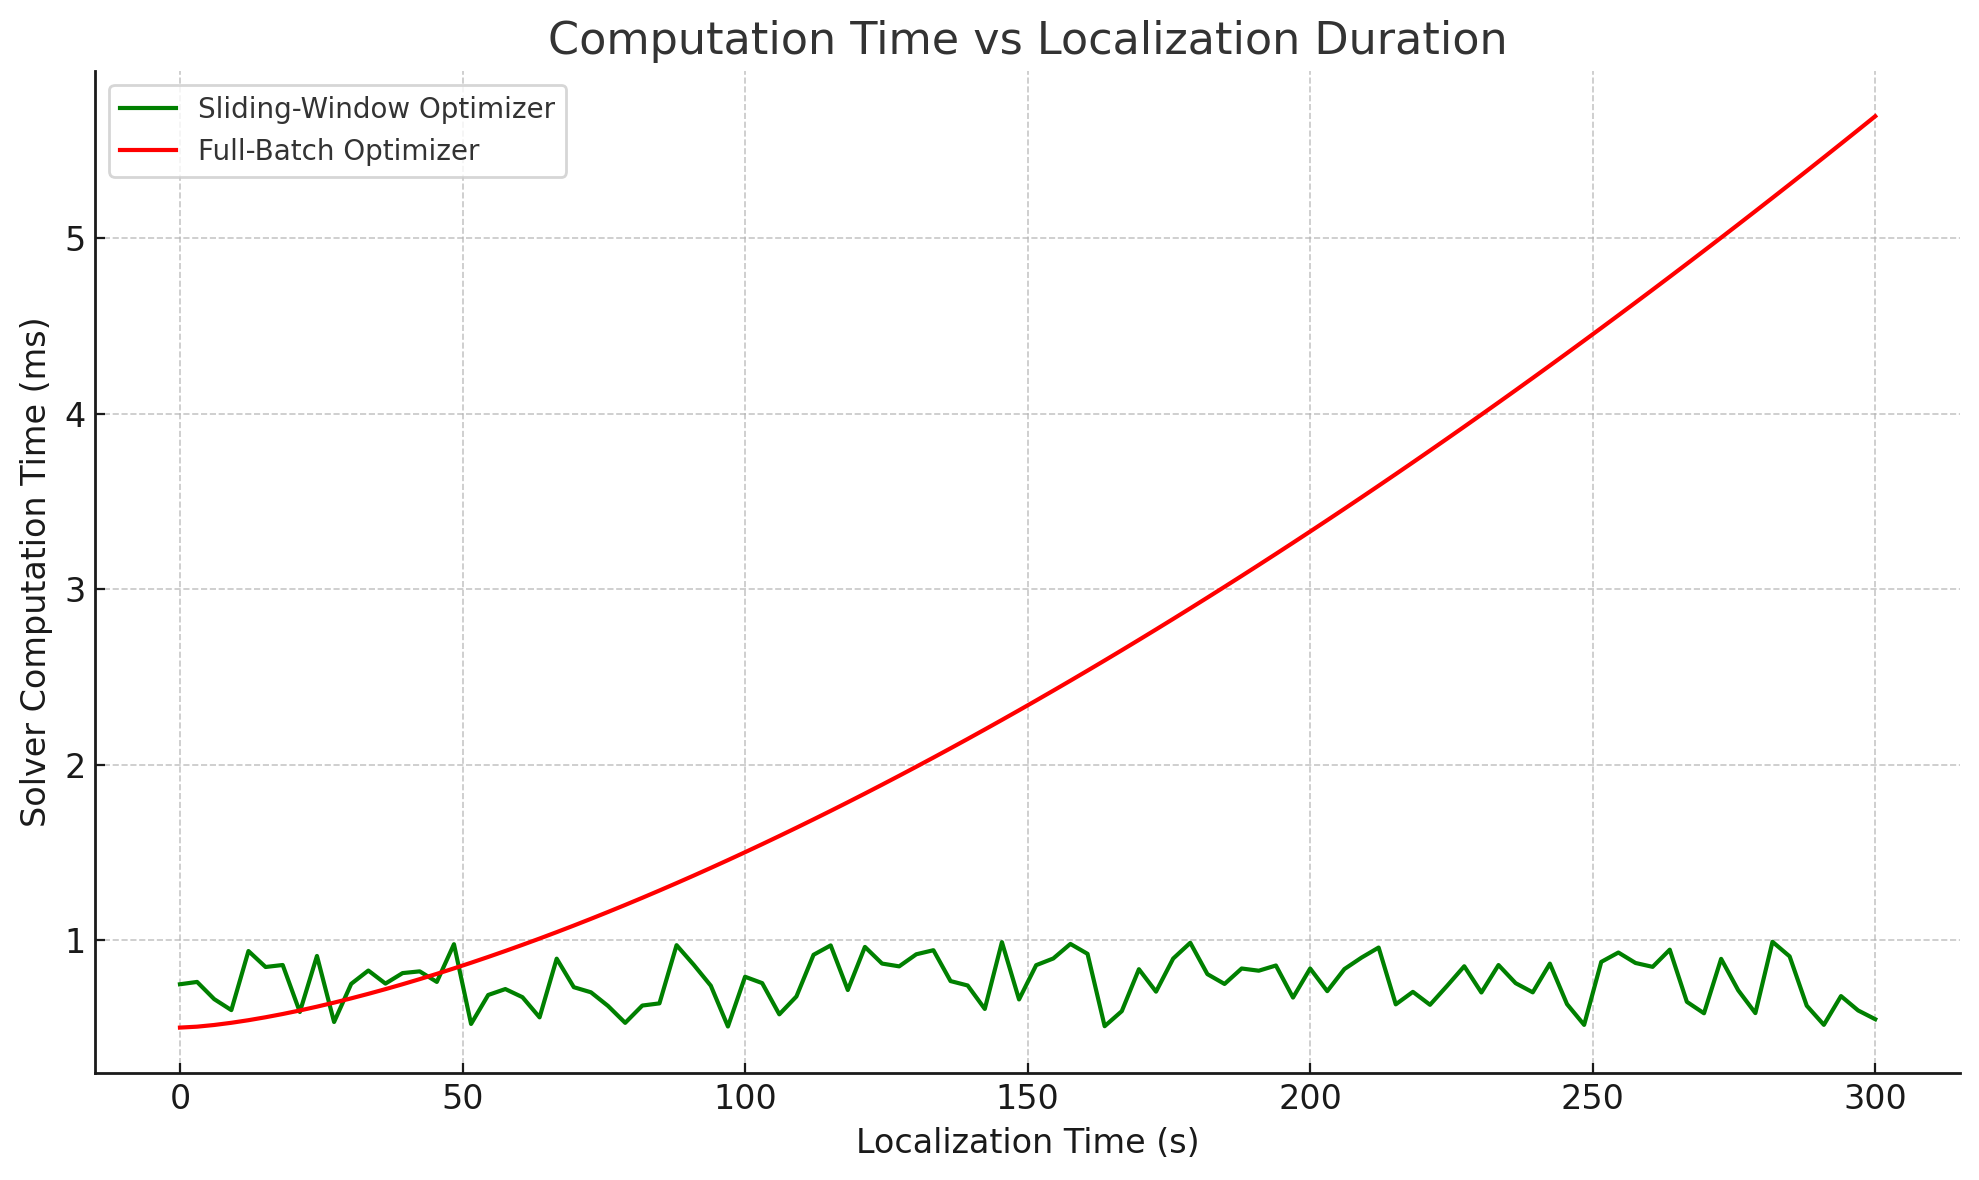
\includegraphics[ width=\linewidth , height=\linewidth]{images/compration_registration_alg.png}
		\caption{Computation time trend of sliding-window vs full-batch optimizer.}
		\label{fig:sliding_vs_batch}
	\end{subfigure}
	\hfill
	\begin{subfigure}[t]{0.48\textwidth}
		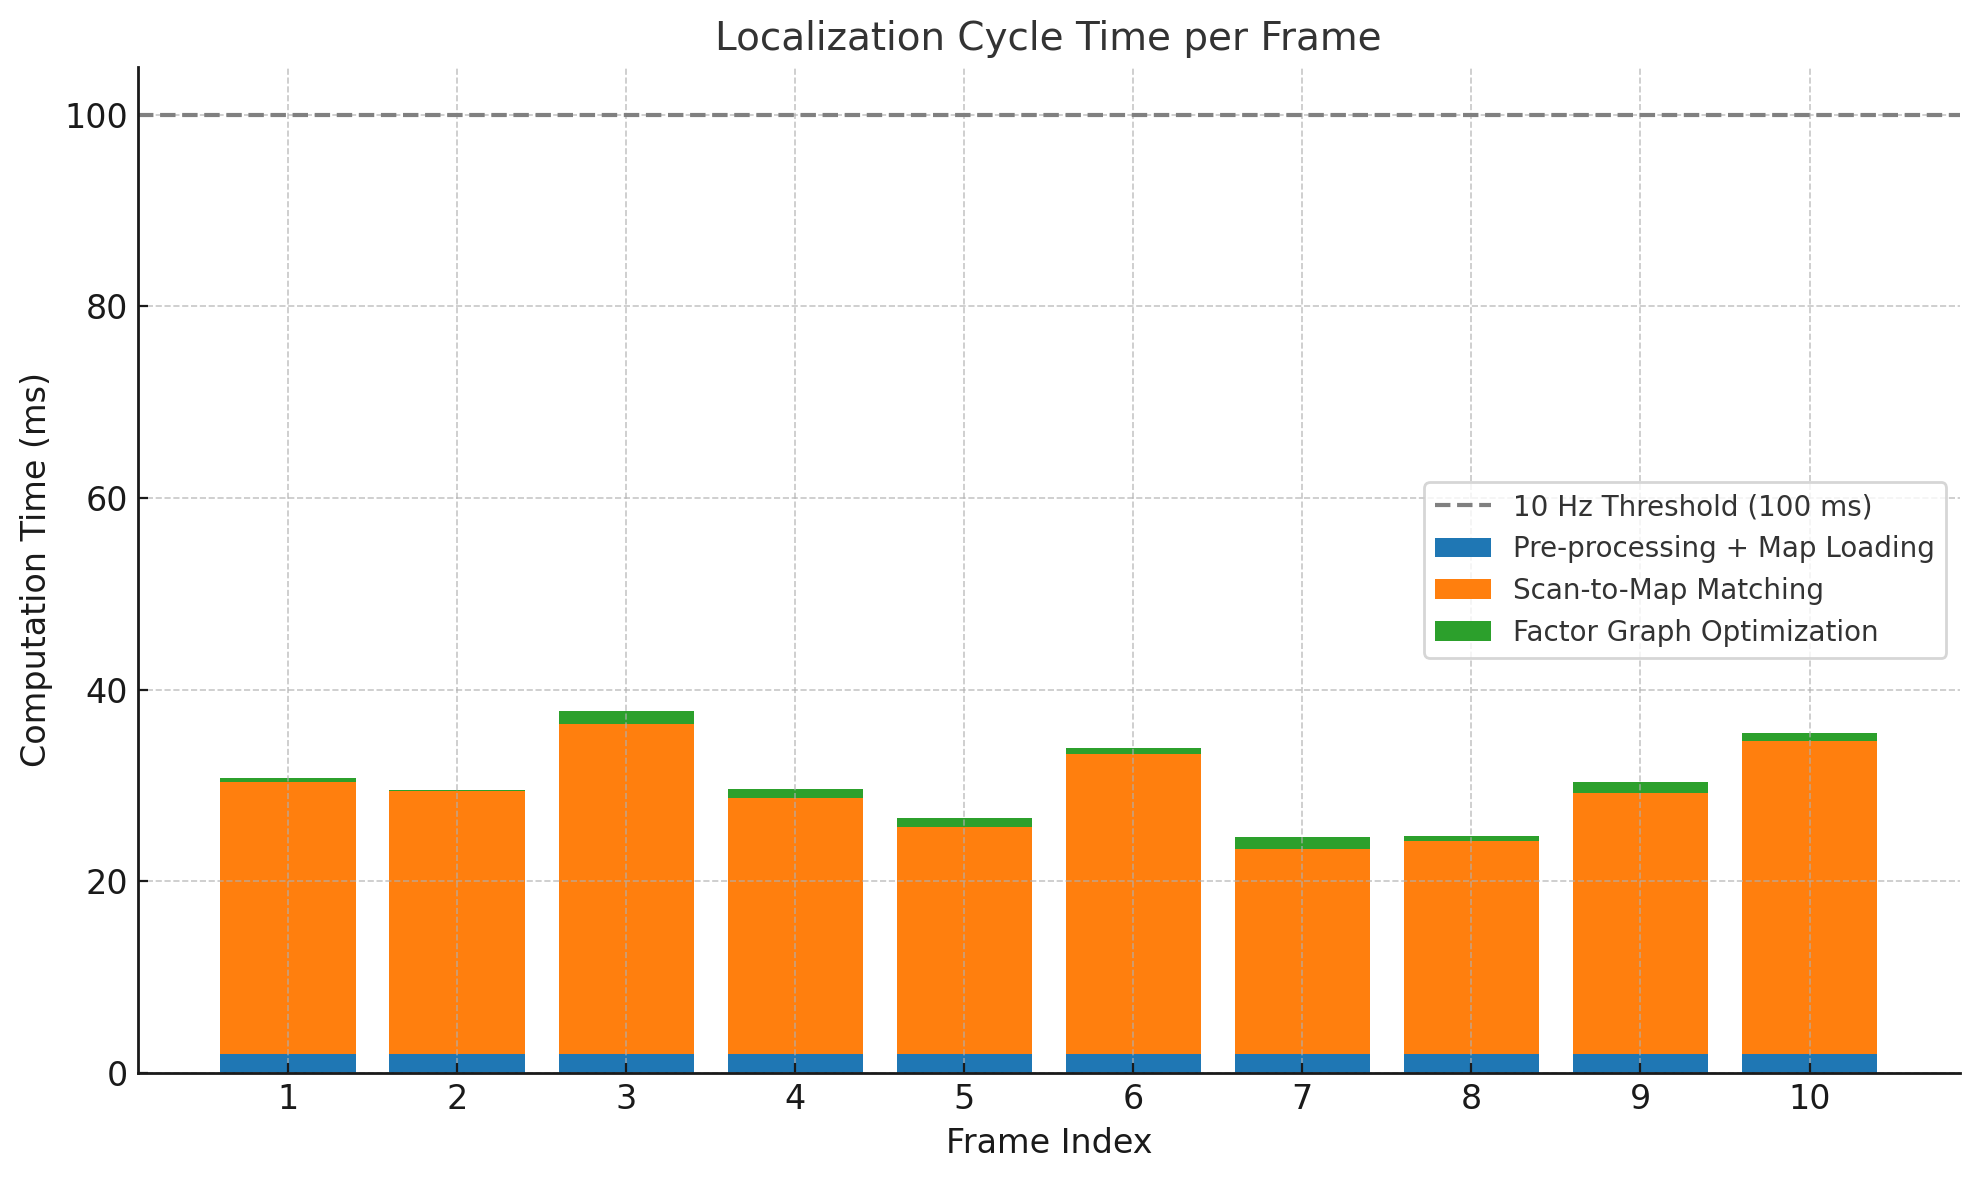
\includegraphics[width=\linewidth ,height=\linewidth]{images/localization_cycle.png}
		\caption{Computation time breakdown per frame (stacked components).}
		\label{fig:computation_summary}
	\end{subfigure}
	\caption{Computation characteristics of the proposed localization system: Sliding-window optimization scalability and real-time frame-wise timing breakdown.}
	\label{fig:computation_summary}
\end{figure}



Considering a high-frequency LiDAR-inertial odometry (LIO) stream and periodic map-matching updates, we compare a sliding-window factor-graph optimizer against a full-batch solver. By restricting the graph to the most recent 5–50 seconds of data,as shown in Figure~\ref{fig:sliding_vs_batch} the sliding-window approach maintains nearly constant solve times under 1 ms per update regardless of localization duration. In contrast, the full-batch solver’s complexity grows superlinearly as more keyframes accumulate, eventually fail in real‐time as the numer of nodes increase.

Figure~\ref{fig:computation_summary} further breaks down the per-frame latency of the proposed system. With point-cloud pre-processing and map loading taking ~2 ms, scan-to-map matching ~25 ms, and factor-graph optimization ~1 ms, the total remains below 35 ms. This comfortably satisfies the real-time 10 Hz requirement (100 ms), achieving ~36 Hz processing frequency.

\subsection{ Extended Evaluation Under Challenging Conditions}


\subsubsection{Scenario A – Dynamic Object Removal}

In this evaluation, we assess the impact of incorporating dynamic object removal into the localization pipeline.Example of  detected 3D bounding boxes and the corresponding retained point cloud after dynamic object removal are illustrated in Figure~\ref{fig:dynamic-object-removal}.The objective is to analyze how removing transient objects from LiDAR scans influences registration accuracy, localization robustness, and computational efficiency. Key performance indicators include registration convergence rate, average iteration count and  execution time are evaluated.

\begin{figure}[H]
\centering
\begin{subfigure}[t]{0.47\textwidth}
	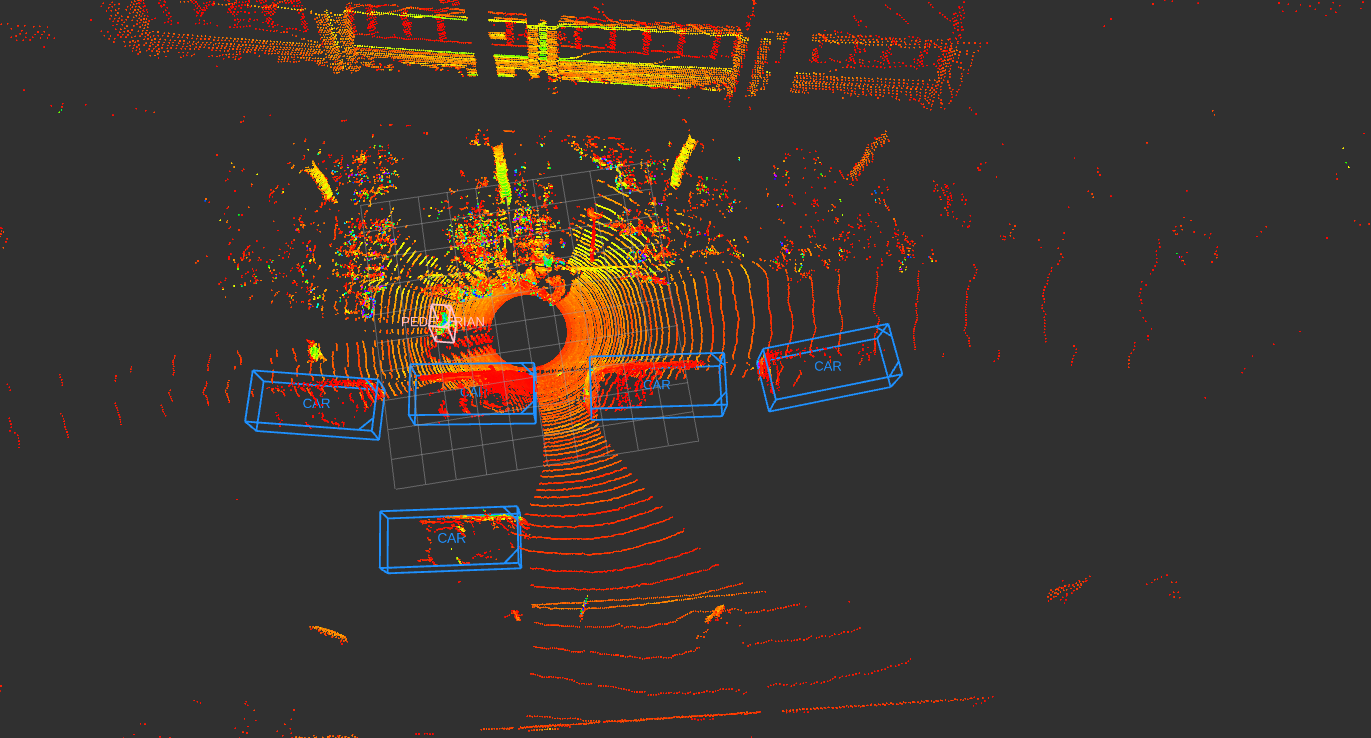
\includegraphics[width=\linewidth]{images/object_detection.png}
	\caption{3D bounding box of detected dynamic objects }
	\label{fig:3d-box-dynamic-object}
\end{subfigure}
\hfill
\begin{subfigure}[t]{0.47\textwidth}
	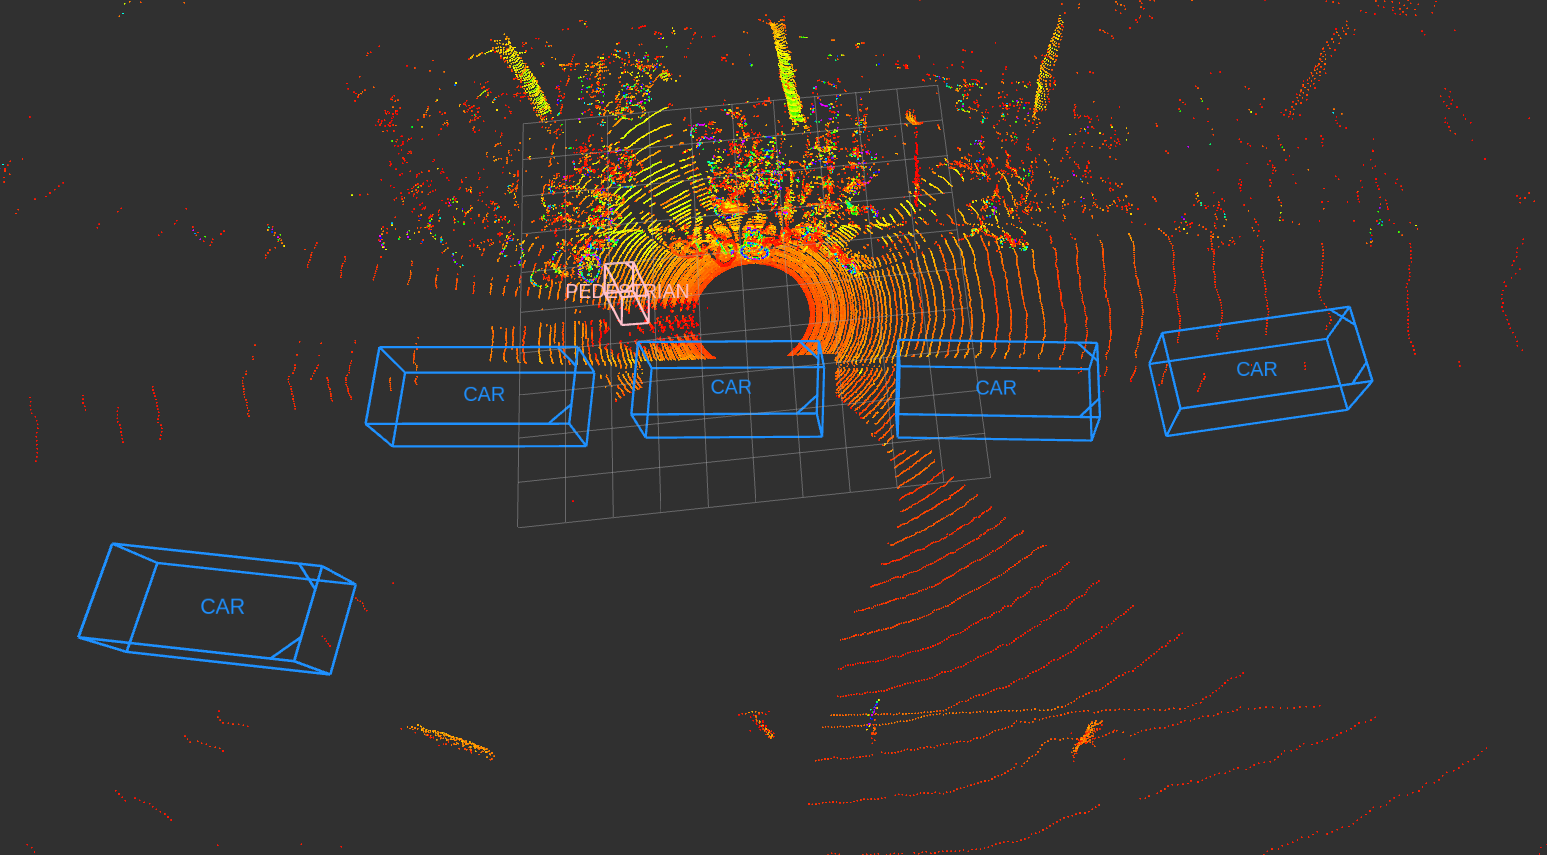
\includegraphics[width=\linewidth]{images/object_detection_remove.png}
	\caption{ Point-cloud retained after removing points with 3d bounding box.
	}
	\label{fig:3d-box-dynamic-object-removal}
\end{subfigure}
\caption[Detecting and removing dynamic objects from 3d LIDAR point-cloud]{Detecting and removing dynamic objects from 3d LIDAR point-cloud.}
\label{fig:dynamic-object-removal}
\end{figure}

\begin{table}[H]
	\centering
	\renewcommand{\arraystretch}{0.4}
	\setlength{\tabcolsep}{10pt}
	\caption{Comparison of Point-cloud Registration Metrics Before and After Dynamic Object Removal}
	\label{tab:dynamic_removal_stats}
	\begin{tabular}{@{}lccc@{}}
		\toprule
		\textbf{Metric} & \textbf{Without Removal} & \textbf{With Removal} & \textbf{Improvement} \\
		\midrule
		Avg. Registration Iterations & 19 & 12  & ↓ 7 \\
		Avg. Execution Time (ms)     & 14.41 & 9.73  & ↓ 4.68 \\
		Registration Failures        & 7     & 2     & ↓ 5 \\
		\bottomrule
	\end{tabular}
\end{table}

\begin{figure}[H]
	\centering
	\begin{subfigure}[t]{0.45\textwidth}
		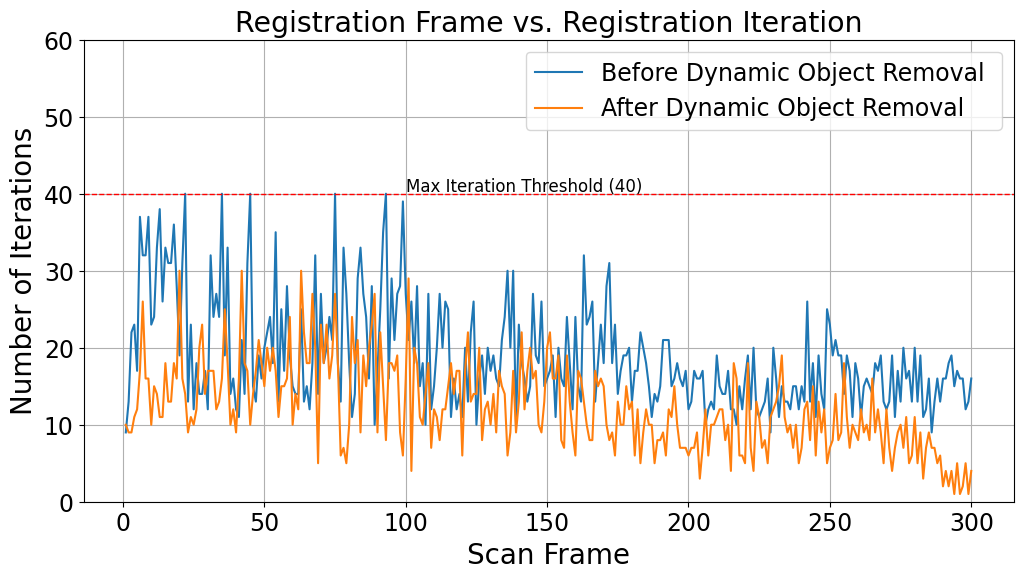
\includegraphics[width=\linewidth]{images/registration_iter_com.png}
		\caption{Registration iterations required per scan frame.}
		\label{fig:reg_iter}
	\end{subfigure}
	\hfill
	\begin{subfigure}[t]{0.45\textwidth}
		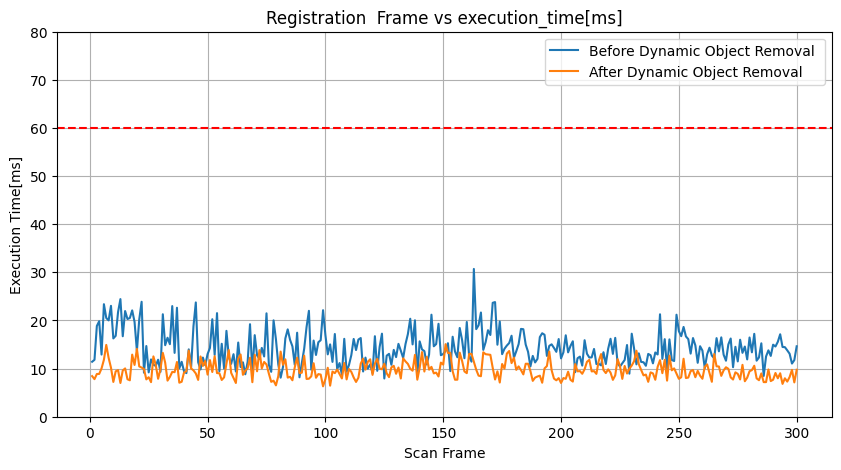
\includegraphics[width=\linewidth]{images/registration_exectime_com.png}
		\caption{Registration Execution time per frame.}
		\label{fig:reg_time}
	\end{subfigure}
	\hfill
	\begin{subfigure}[t]{0.45\textwidth}
		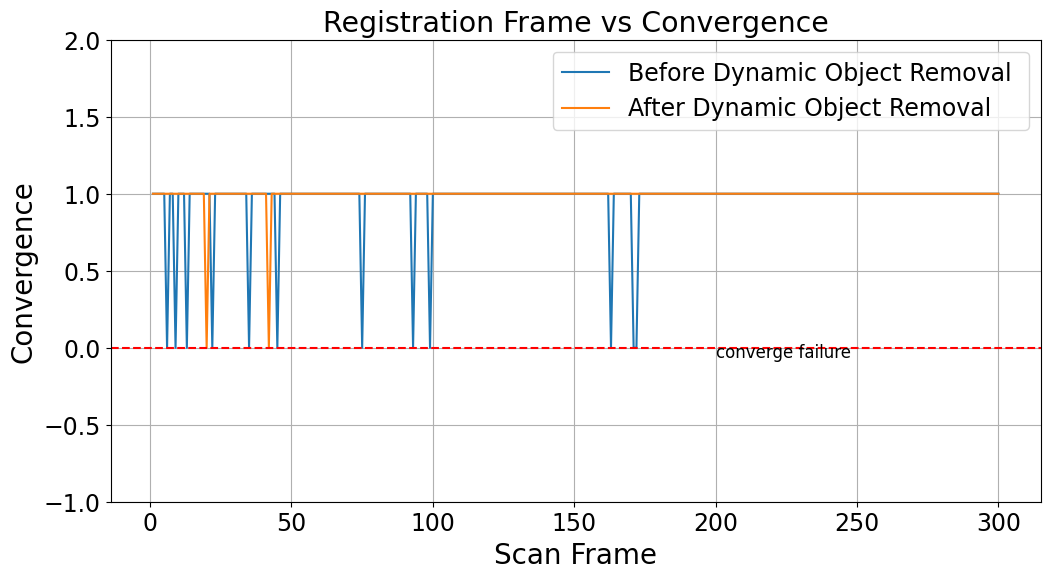
\includegraphics[width=\linewidth]{images/registration_conver_comp.png}
		 \caption{Convergence status (1 = success, 0 = failure) across frames.}
		\label{fig:reg_converge}
	\end{subfigure}
	\caption[Point-cloud Registration Performance with and without Dynamic Object Removal]{\textbf{Registration performance before and after dynamic object removal.} Each subplot shows the impact of removing dynamic objects on and iteration count (a) , execution time (b), and convergence (c). Across 300 frames, the system becomes more stable, efficient, and reliable after filtering out dynamic elements from the scan.}
	\label{fig:registration_metrics_comparison}
\end{figure}

The point-cloud registration performance was evaluated across 300 scan frames before and after applying dynamic object removal. As summarized in Table~\ref{tab:dynamic_removal_stats}, filtering dynamic objects results  reduction in average registration iterations (from 19 to 12) and execution time (from 14.41 ms to 9.73 ms). Additionally, the number of convergence failures dropped from 7 to 2. The performance plots in Figure~\ref{fig:registration_metrics_comparison} further illustrate this trend. Dynamic object removal improves stability and efficiency by eliminating noisy inputs that otherwise increase iteration count, processing time, or lead to failed alignments.


Table~\ref{tab:dynamic_object_runtime_pipeline_comparison} presents the computational overhead introduced by integrating dynamic object detection and filtering into the localization pipeline. While this module enhances registration robustness and accuracy, it incurs additional processing time. Specifically, the 3D object detection step (using ONNX inference) adds approximately 31 ms, and the point cloud filtering (using a CropBox filter) adds another 8 ms per frame. Although the registration and optimization stage benefits from a reduction in processing time—from 15 ms to 10 ms—the overall per-frame runtime increases from 15 ms (without removal) to 49 ms (with removal), resulting in a net overhead of 34 ms. Despite this increase, the system remains within acceptable real-time performance bounds for medium-speed mobile robotics applications.


\begin{table}[H]
	\centering
	\renewcommand{\arraystretch}{0.3}
	\setlength{\tabcolsep}{3pt}
	\caption{Per-frame runtime analysis with and without dynamic object removal.}
	\label{tab:dynamic_object_runtime_pipeline_comparison}
	\begin{tabular}{lccc}
		\toprule
		\textbf{Component} & \textbf{Without Removal (ms)} & \textbf{With Removal (ms)} & \textbf{Overhead(ms)} \\
		\midrule
		Object Detection         & —     & 31.0  & +31.0 \\
		Point Cloud Filtering    & —     & 8.0   & +8.0 \\
		Registration and other            & 15.0  & 10.0   & ↓ 5 \\
		\midrule
		\textbf{Total}           & 15.0  & 49.0  & +34.0 \\
		\bottomrule
	\end{tabular}
\end{table}



\subsubsection{Scenario B – Map-Side Feature-Sparse Environment}

Map-side feature-sparse environments refer to areas where the current LiDAR observations contain few or no correspondences in the prebuilt map. This situation typically arises at the boundaries of a mapped area, in unmapped zones, or at transitions between separately built or merged submaps. In such regions, the prior map lacks persistent geometric features required for reliable scan-to-map registration, resulting in degraded or failed localization if scan matching is used in isolation.

\begin{figure}[H]
	\centering
	\begin{tikzpicture}		
		% Main trajectory image
		\node[anchor=south west, inner sep=0] (main) at (0,0)
		{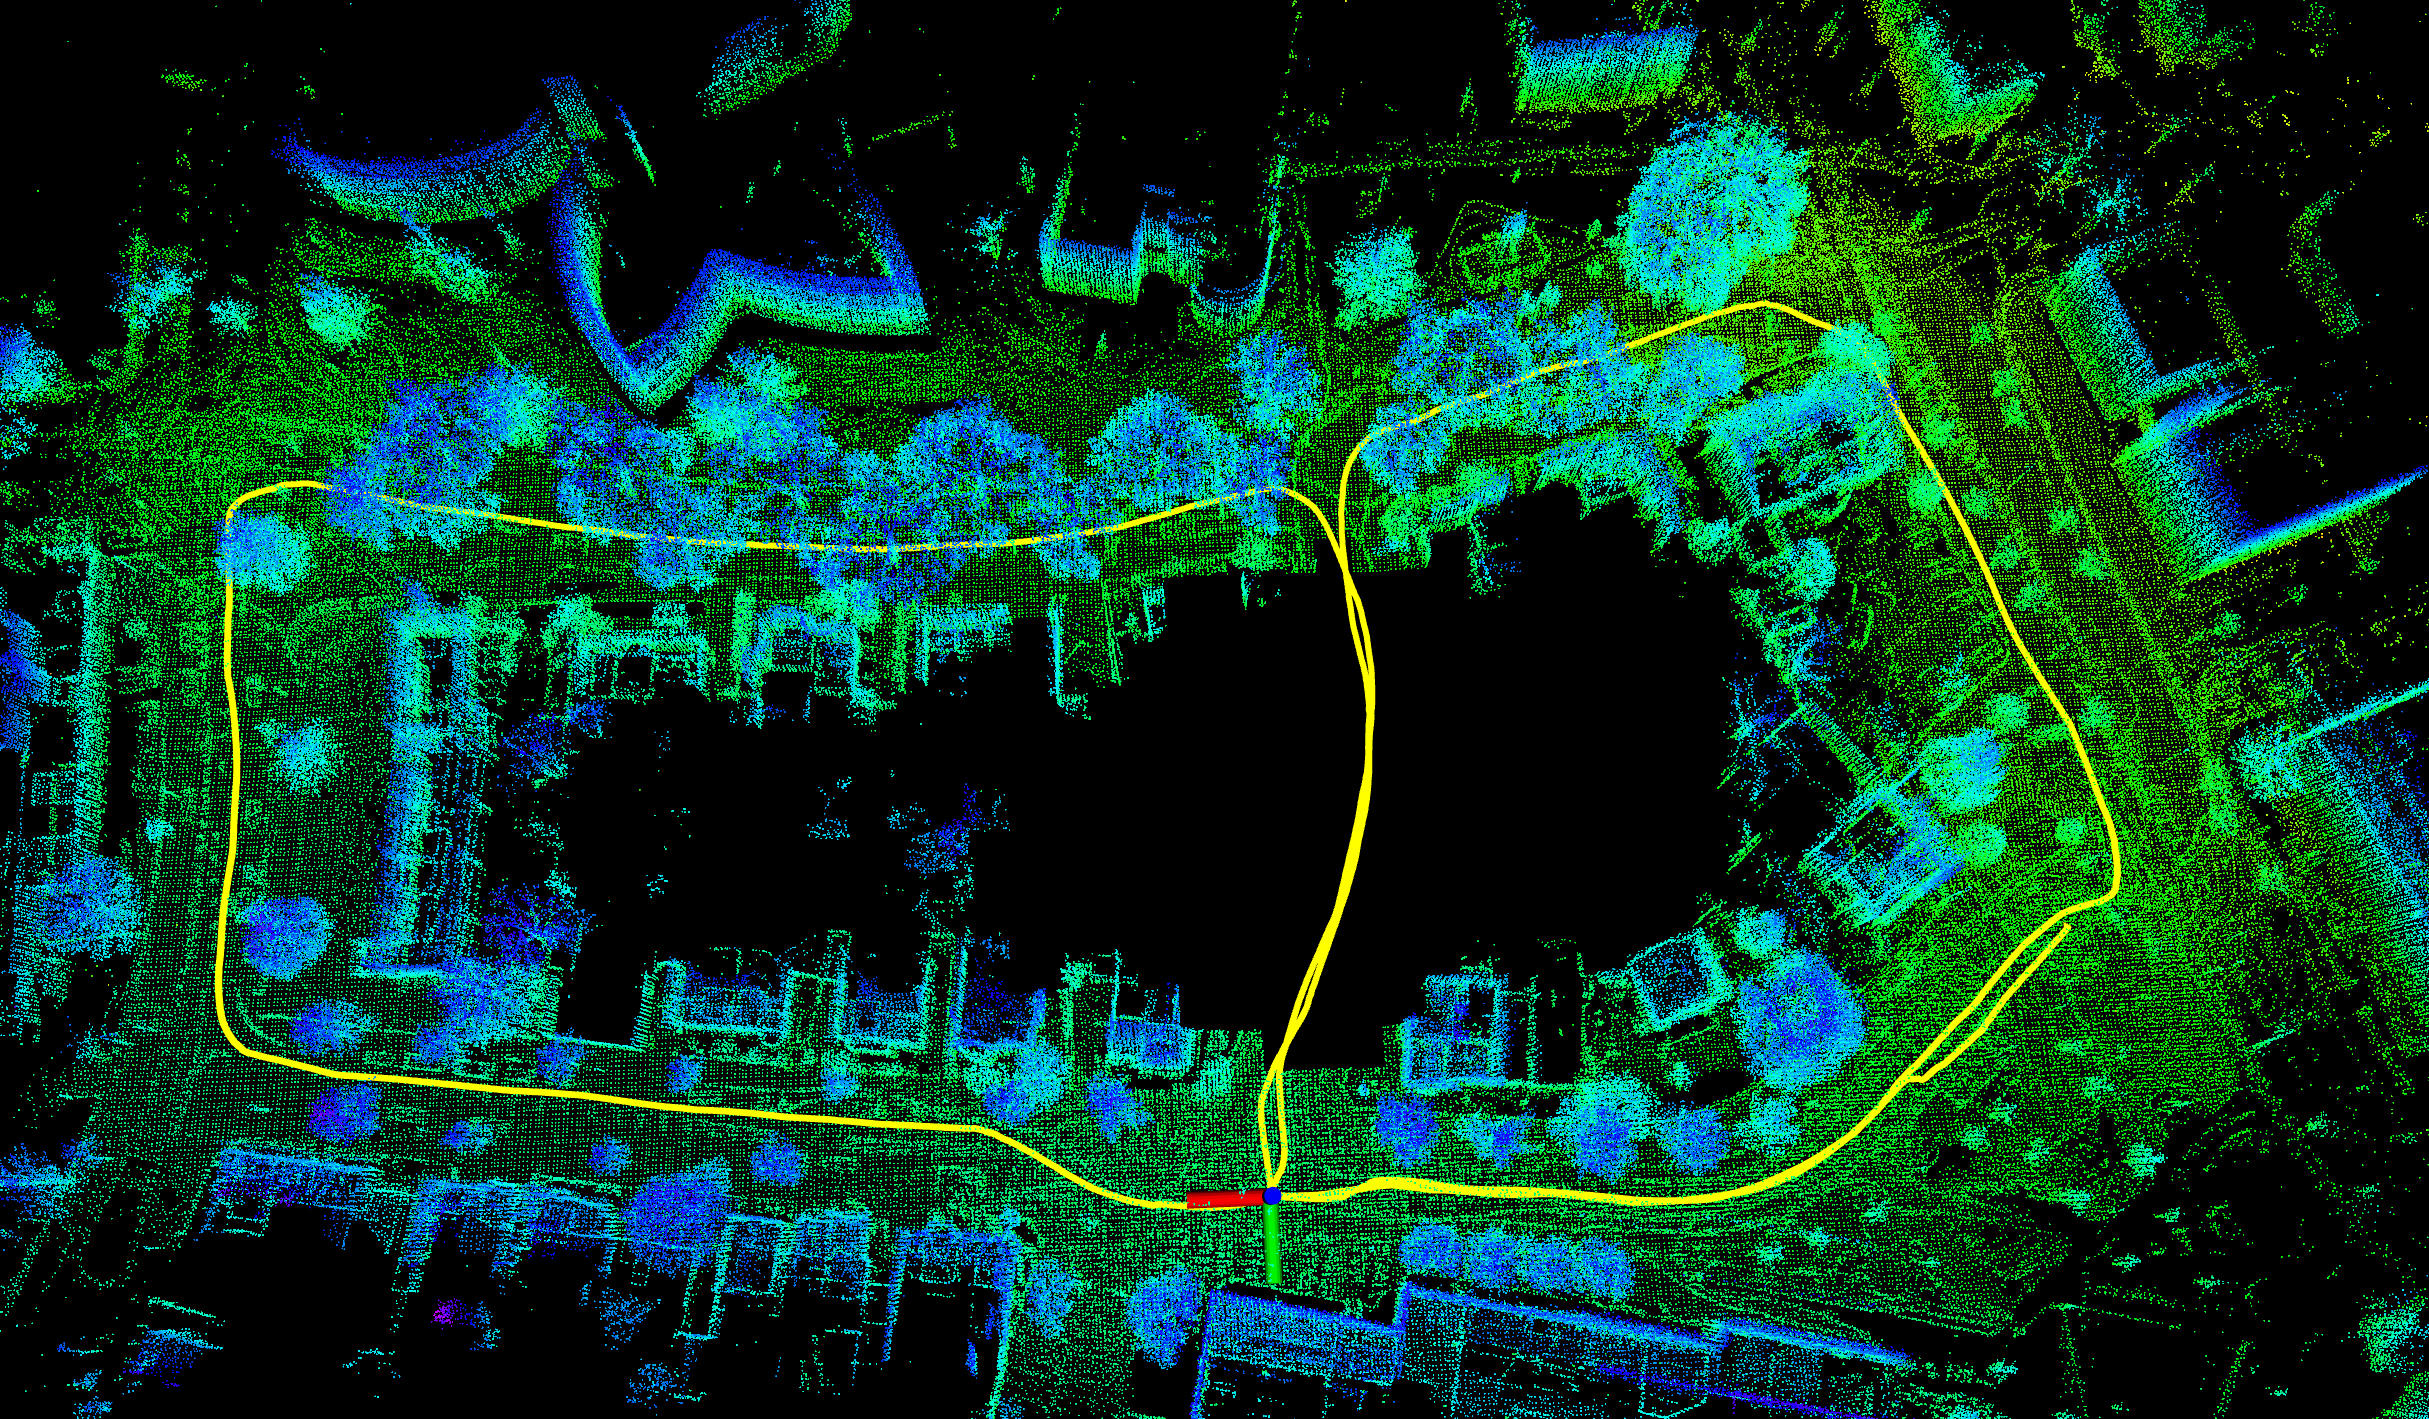
\includegraphics[width=0.6\textwidth]{images/unmapped_zone2.png}};
		% Coordinate system normalized to the image
		\begin{scope}[x={(main.south east)}, y={(main.north west)}]
			% Red dashed rectangle for zoom box (adjust coordinates!)
			\draw[red, line width=1.5pt, dash pattern=on 4pt off 2pt] (0.48, 0.25) rectangle (0.59, 0.58);
			% Red arrow from zoom box o tzoomed-in image
			\draw[->, red, thick] (0.95, 0.55) -- (0.97, 0.57);
			% Add label above the rectangle
			\node[white] at (0.535, 0.41) {transition zone: 70m};
		\end{scope}
		
		
		
	\end{tikzpicture}
	
	\caption[]%
	{\textbf{	Localization in transition zone.} The robot enters a transition region (highlighted in red) where LiDAR scan matching fails due to the absence of stable features in the prebuilt map
	}
	\label{fig:unmapped-zone}
\end{figure}

In this scenario, the robot traverses an approximately 70-meter-long transition sub-street connecting two main streets, which includes partially mapped and unmapped segments. As shown in Figure~\ref{fig:unmapped-zone}, this zone is highlighted in red. This path was repeated twice to validate consistency. The NDT-based scan matching frequently failed within this zone due to the lack of map overlap, as reflected in the significant error spikes shown in Figure~\ref{fig:ape-error-unmapped-ndt}, \ref{fig:ape-error-trajectory-unmapped-proposed}. However, the proposed fusion pipeline maintained stable localization throughout the traversal shown in Figure~\ref{fig:ape-error-unmapped-proposed}.

A comparison of APE statistics is summarized in Table ~\ref{tab:ape-unmapped-comparison} . Notably, the maximum APE for NDT Scan Matching reached 2.178 meters, whereas the proposed fusion method limited the maximum error to 0.455 meters. The Root Mean Square Error (RMSE) also showed a significant reduction, from 0.295 meters in NDT to 0.095 meters in the fusion approach. These results underscore the robustness of the proposed method in feature-deprived environments.


For context, under standard conditions specifically, Saxion Sequence 1 APE statistics is summarized in Table ~\ref{tab:ape_rot_saxion_seq1}, which was conducted in a fully mapped environment the proposed fusion method achieved a maximum APE of 0.395 meters and an RMSE of 0.067 meters. This comparison underscores the robustness of the fusion approach, demonstrating its ability to maintain localization accuracy even in challenging, feature-sparse environments.

\begin{figure}[H]
	\centering
	\begin{subfigure}[t]{0.49\textwidth}
		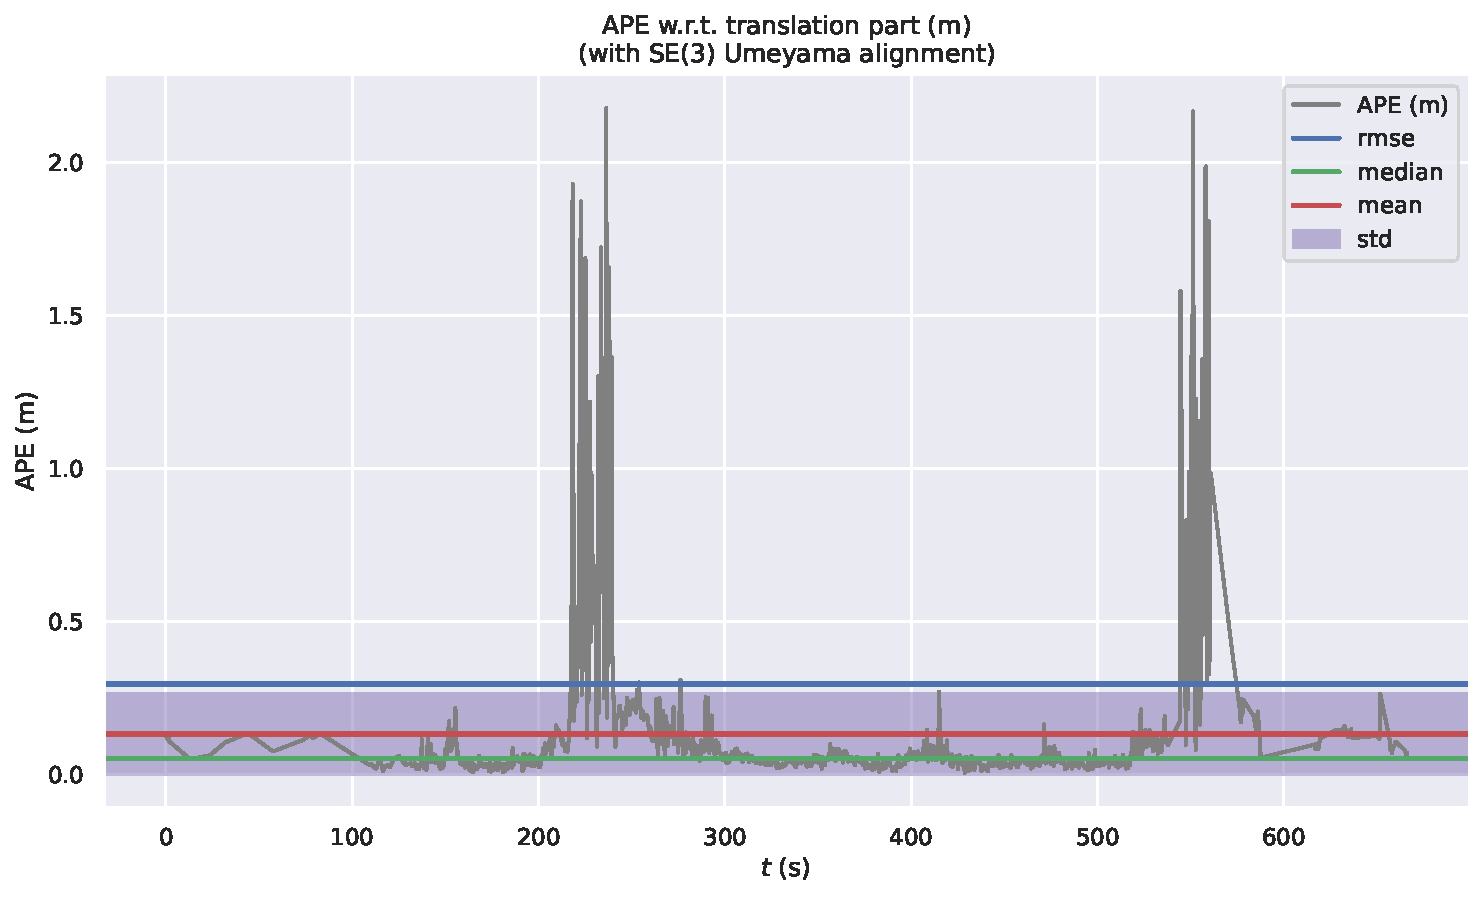
\includegraphics[width=\linewidth]{images/unmappedzone_error_ndt2.pdf}
		\caption{ NDT Scan Matching  APE - translation part  }
		\label{fig:ape-error-unmapped-ndt}
	\end{subfigure}
	\hfill
	\begin{subfigure}[t]{0.49\textwidth}
		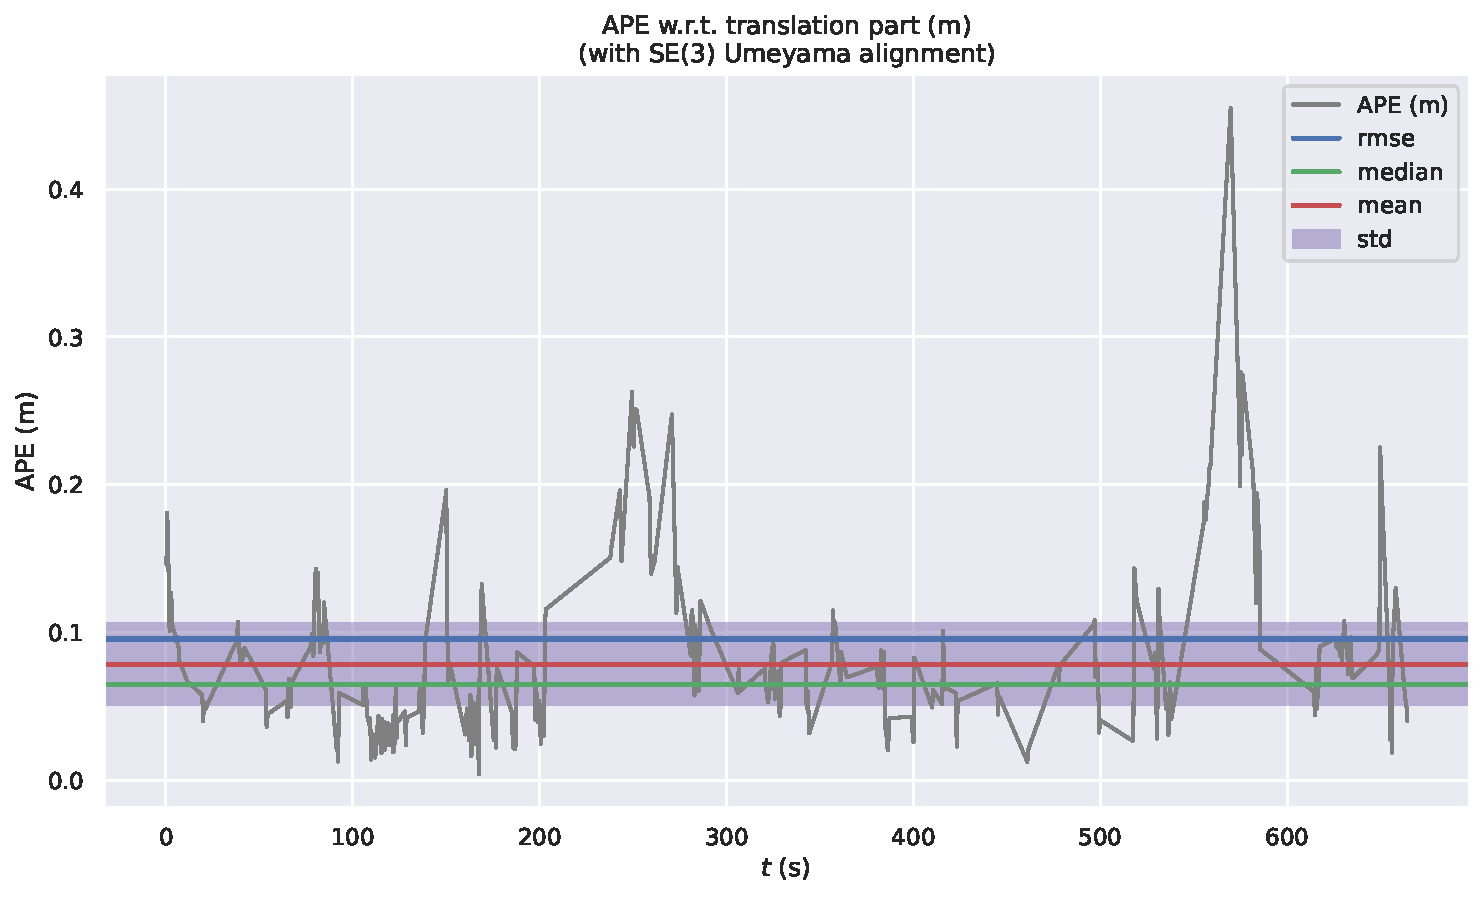
\includegraphics[width=\linewidth]{images/unmapped_zone_error_fused.pdf}
		\caption{ Proposed - translational part
		}
		\label{fig:ape-error-unmapped-proposed}
	\end{subfigure}
    \begin{subfigure}[t]{0.49\textwidth}
    	\includegraphics[page=2 ,width=\linewidth]{images/unmappedzone_error_ndt2.pdf}
    	\caption{ NDT Scan Matching APE Trajectory  - translation part.
    	}
    	\label{fig:ape-error-trajectory-unmapped-proposed}
    \end{subfigure}
	\caption[Error compression  localization in transition zone]{
	\textbf{Error compression  localization in transition zone} The APE for NDT scan matching(a) , Proposed(fusion)(b) and NDT APE trajectory(c)}
	\label{fig:ape-error-unmapped}
\end{figure}

\begin{table}[H]
	\centering
	\caption{Absolute Pose Error (APE) Statistics in Transition Corridor}
	\label{tab:ape-unmapped-comparison}
	\begin{tabular}{lcccc}
		\toprule
		\textbf{Method} & \textbf{Max APE (m)} & \textbf{Mean APE (m)} & \textbf{RMSE (m)} & \textbf{Std Dev (m)} \\
		\midrule
		Proposed Fusion   &\textbf{ 0.455} & \textbf{0.078} & \textbf{0.095} &\textbf{ 0.054} \\
		NDT Scan Matching & 2.178 & 0.131 & 0.295 & 0.264 \\
		FAST-LIO2   & 7.59 & 1.456  & 2.197 & 1.645 \\
		
		
		\bottomrule
	\end{tabular}
{\footnotesize \textit{Note:} Bold values indicate the best performance across each metric.}
\end{table}


\subsubsection{Scenario C – Recent-Map under Composite Environmental Noise}

In this scenario we evaluate localization performance using a one-month-old prebuilt map and subject the live LiDAR observations to three levels of composite geometric noise (Mild, Moderate, Severe, see Table~\ref{tab:noise_levels}). Figure \ref{fig:different-noise-levels} presents  bird’s-eye views of the same point cloud under each noise level, illustrating point dropouts, scatter, backscatter shifts, and spurious returns. After adding the selected noise level, we test the localization pipeline and compare the resulting Absolute Pose Error (APE) against the standard baseline, thereby isolating the pure geometric impact of simulated fog, rain, and snow–like disturbances on localization accuracy.


\begin{figure}[H]
	\centering
	\begin{subfigure}[t]{0.46\textwidth}
		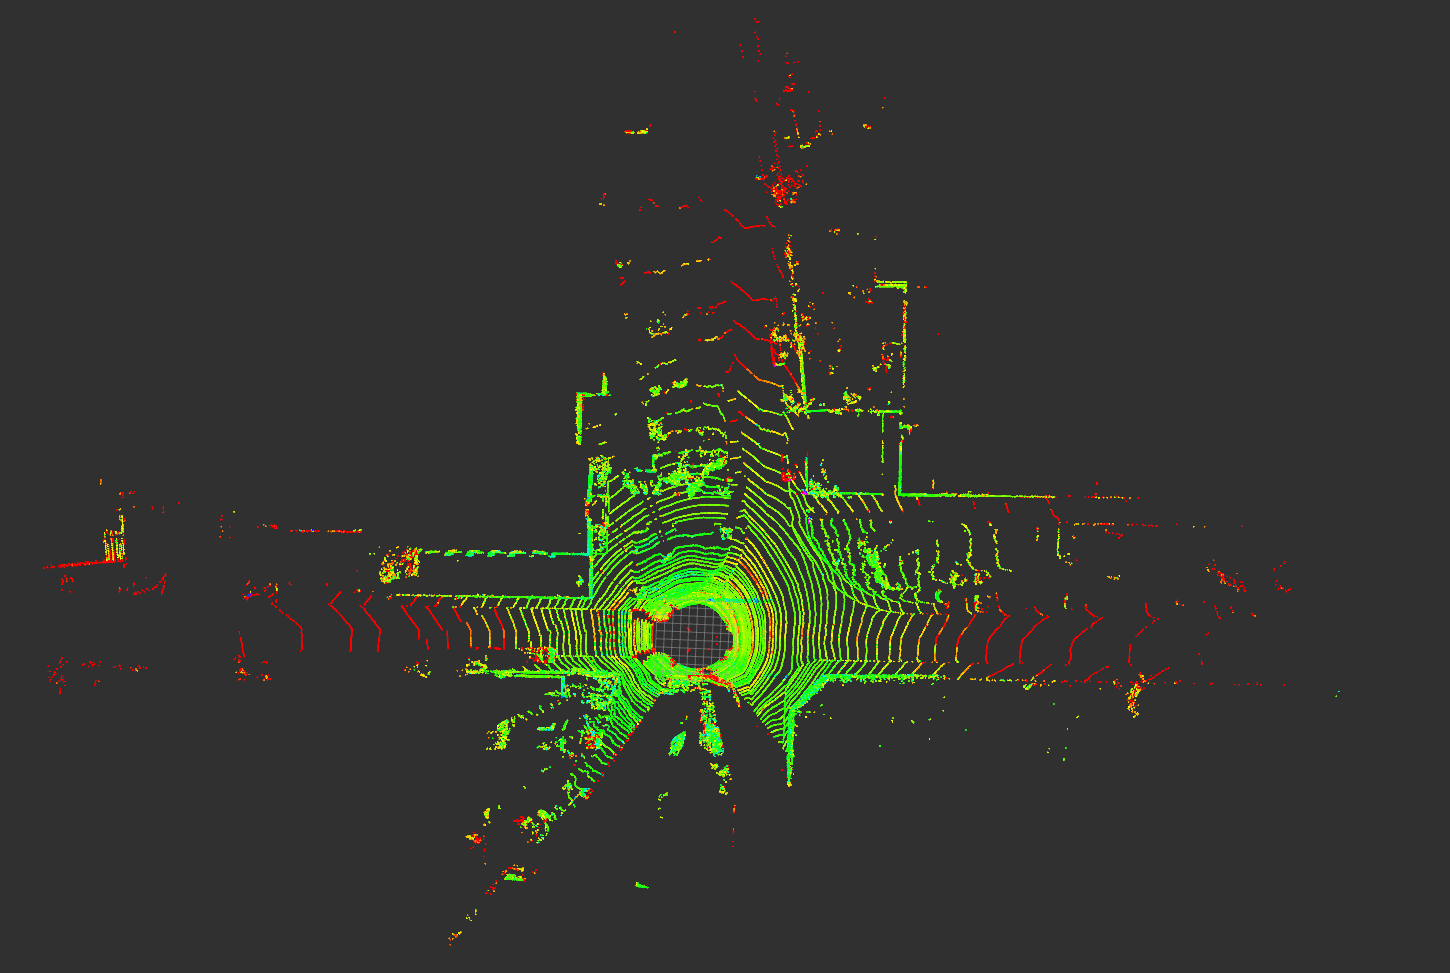
\includegraphics[ height=3.5cm , width=\linewidth]{images/original_pointcloud.png}
		\caption{ Original Point-cloud }
		\label{fig:original-noise-level-pointcloud}
	\end{subfigure}
	\hfill
	\begin{subfigure}[t]{0.46\textwidth}
		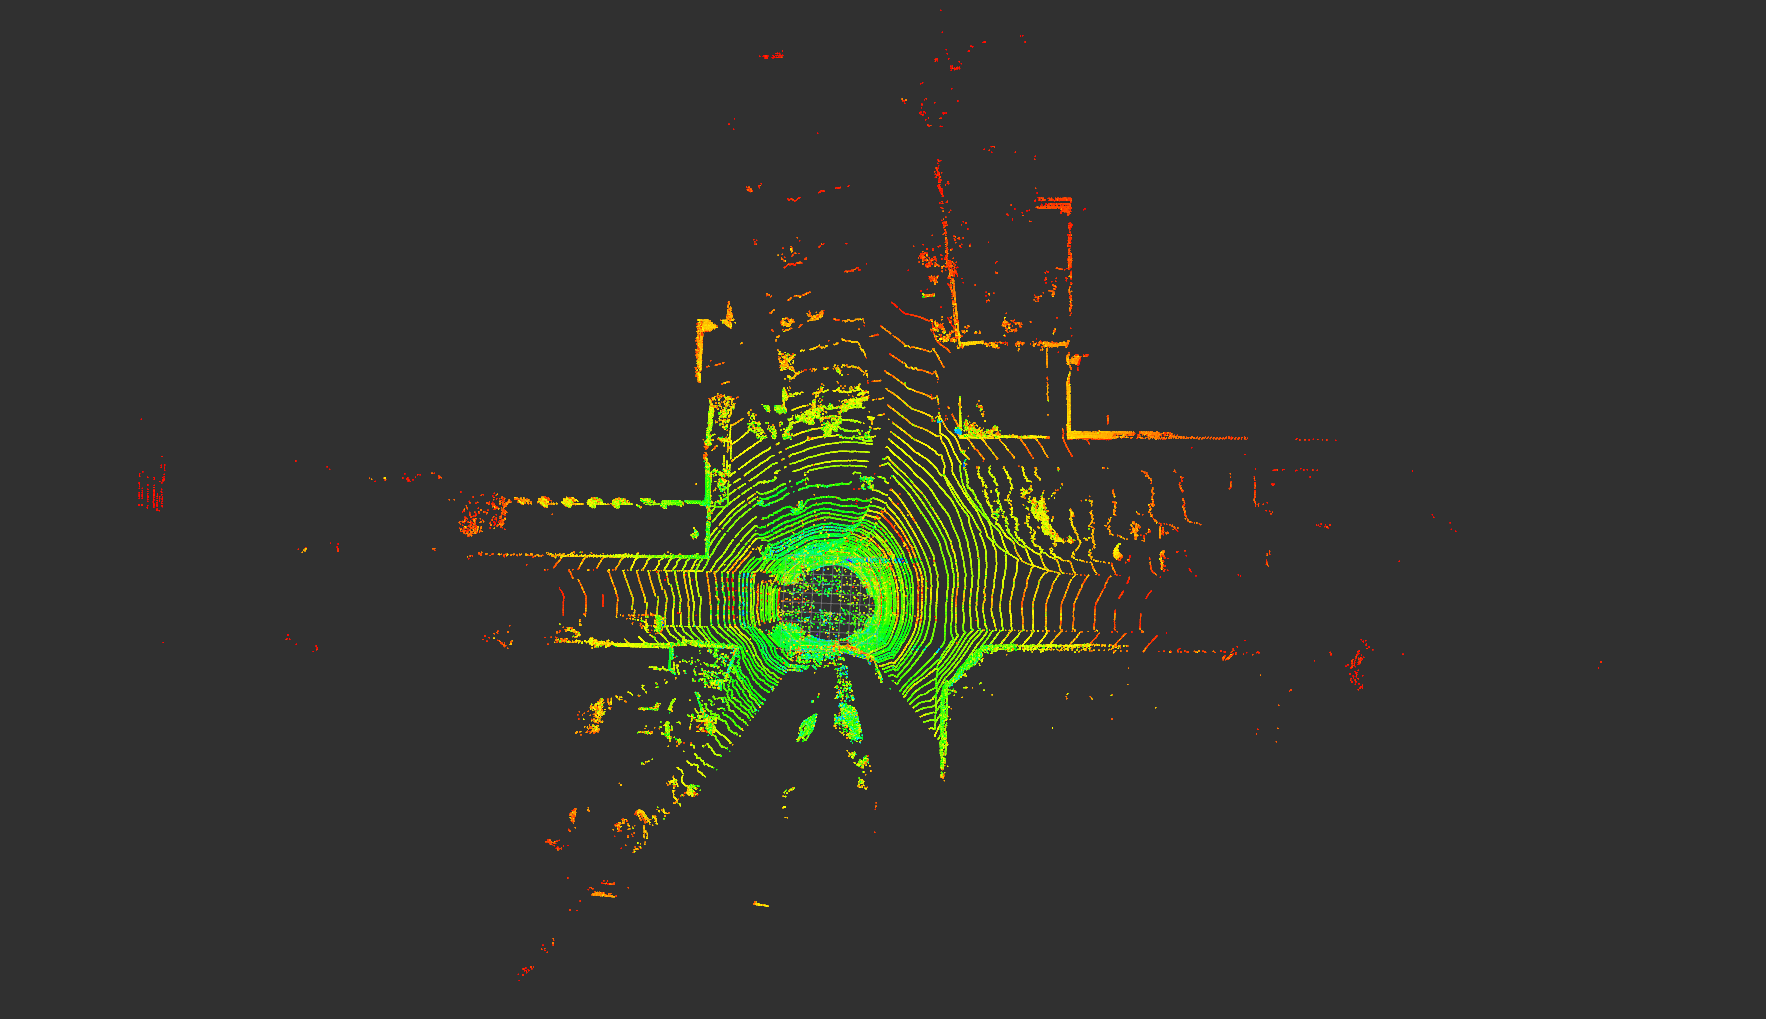
\includegraphics[height=3.5cm , width=\linewidth]{images/level1_noisea.png}
		\caption{ Mild noise level added point-cloud
		}
		\label{fig:mild-noise-level-pointcloud}
	\end{subfigure}
     \hfill
	\begin{subfigure}[t]{0.46\textwidth}
		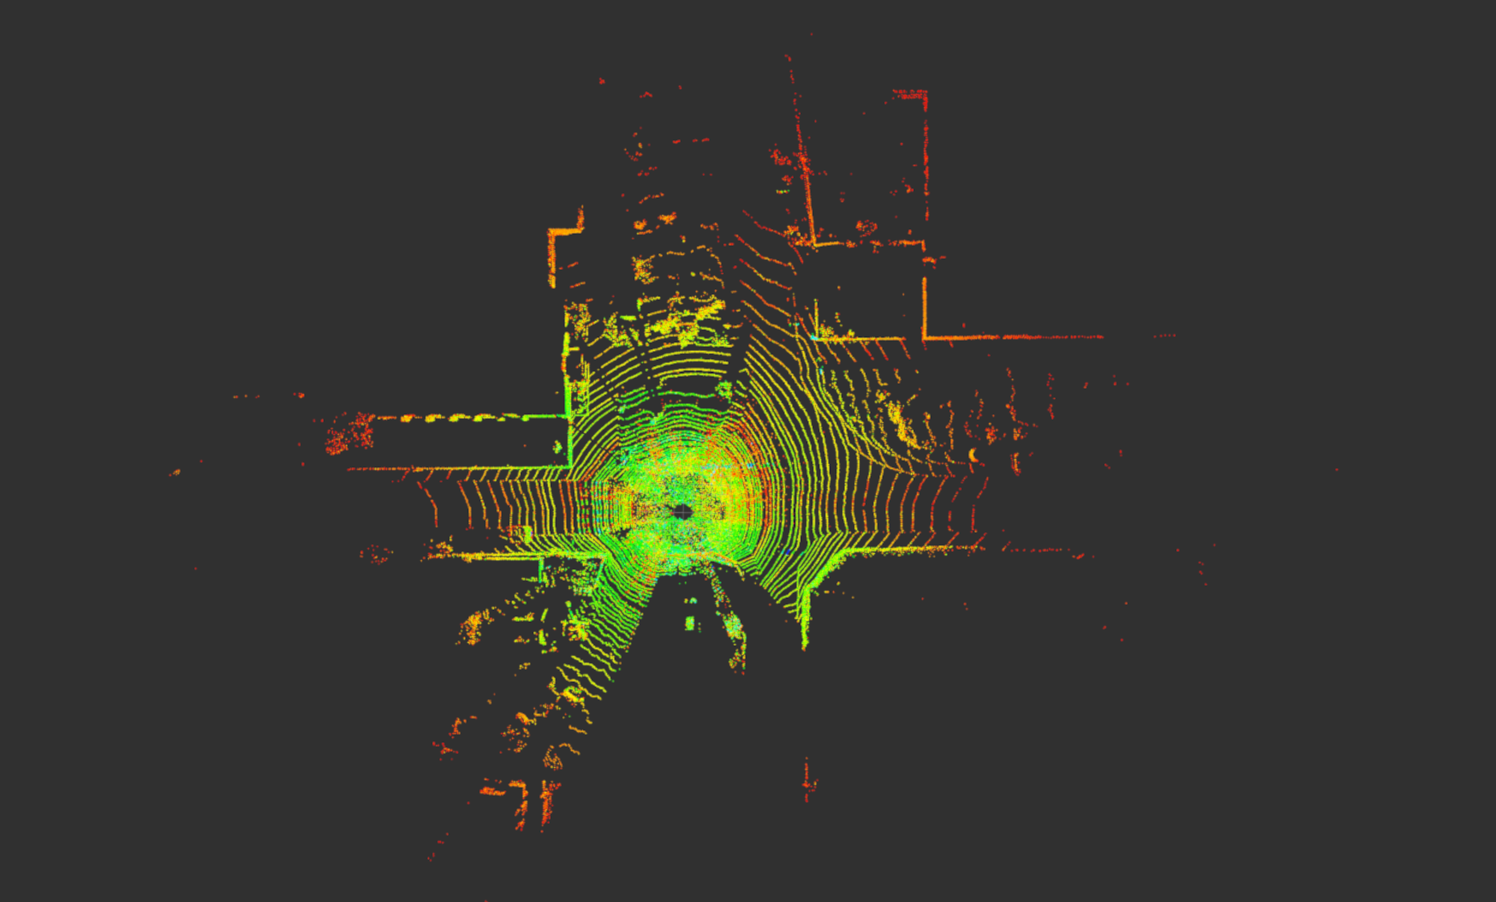
\includegraphics[height=3.5cm , width=\linewidth]{images/level2_noise.png}
		\caption{ Moderate noise level added point-cloud
		}
		\label{fig::mild-noise-level-pointcloud}
	\end{subfigure}
      \hfill
	\begin{subfigure}[t]{0.46\textwidth}
		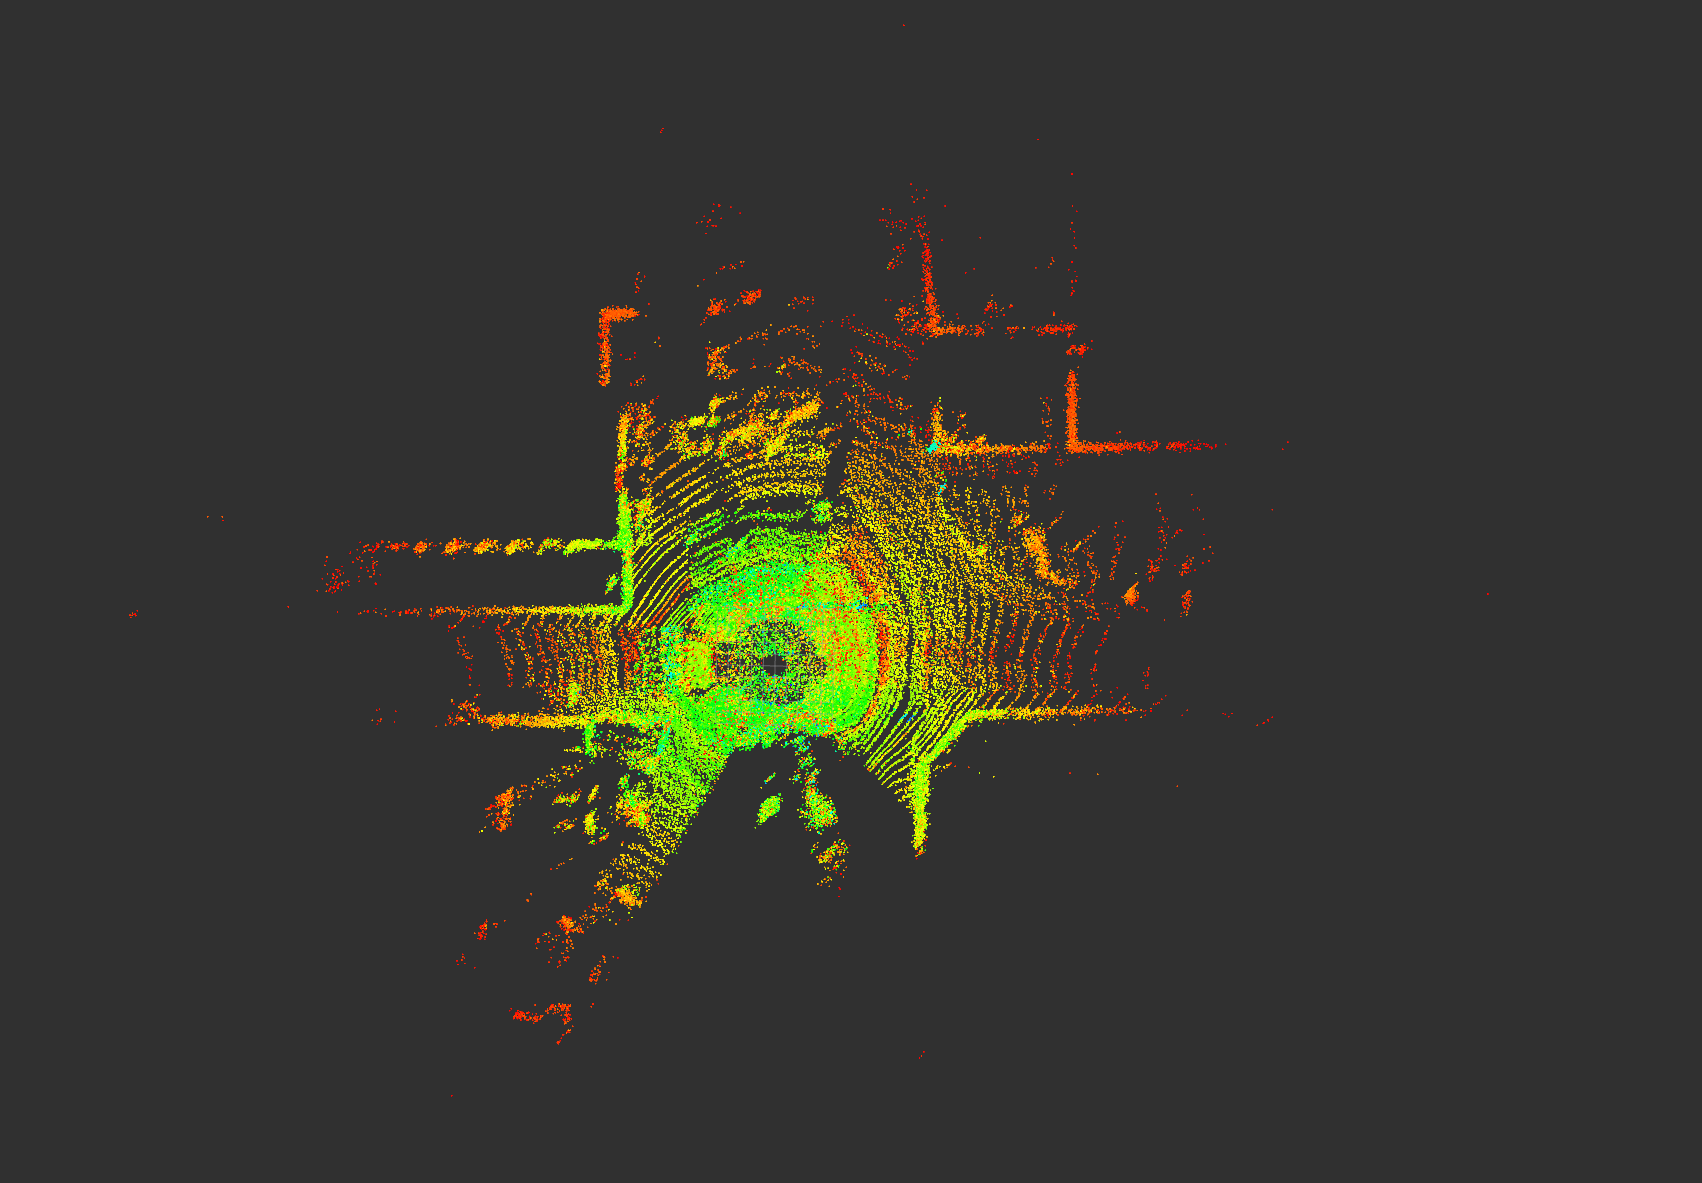
\includegraphics[height=3.5cm , width=\linewidth]{images/level3_noiseb.png}
		\caption{ Severe noise level added point-cloud
		}
		\label{fig:mild-noise-level-pointcloud}
	\end{subfigure}
		
	\caption{Point‐cloud snapshots under increasing composite geometric noise levels: (a) Original scan; (b) Mild noise; (c) Moderate noise; (d) Severe noise.}
	
	\label{fig:different-noise-levels}
\end{figure}

Evaluated on the Saxion Sequence 1 dataset, both Mild and Moderate composite‐noise scenarios incur only minor degradations in translational accuracy on the order of a few centimeters (0.06–0.08 m) compared to the noise free baseline (Table \ref{tab:ape_rot_saxion_seq1}). This demonstrates that both the standalone NDT scan‐matching pipeline and our fusion method remain robust under light to moderate noise level. By contrast, under Severe noise the NDT pipeline intermittently fails, with its maximum translational error exceeding 1.4 m and an overall RMSE of 0.218 m. Our fusion approach, however, still confines drift to acceptable bounds, limiting its maximum APE to 0.38 m and achieving an RMSE of 0.145 m as shown in Figure \ref{fig:different-noise-levels-ate}.

\begin{table}[H]
	\centering
	\caption{Translation (APE) and Rotation Error statistics under Mild, Moderate, and Severe composite noise}
	\label{tab:ape_noise_all_swapped}
	\begin{tabular}{l l l c c c c c}
		\toprule
		\textbf{Condition} & \textbf{Method} & \textbf{Metric}  & \textbf{Max} & \textbf{Mean} & \textbf{Min} & \textbf{RMSE} & \textbf{Std Dev} \\
		\midrule
		\multirow{4}{*}{Mild}     
		& \multirow{2}{*}{NDT}      
		& APE (m)      & 0.4236 & 0.1183 & 0.0163 & 0.1259 & 0.0430 \\
		&                           
		& Rot.\ (deg)  & 5.7259 & 0.4643 & 0.0430 & 0.6845 & 0.5030 \\
		\cmidrule{2-8}
		& \multirow{2}{*}{Proposed} 
		& APE (m)      & 0.3670 & 0.1030 & 0.0186 & 0.1122 & 0.0445 \\
		&                           
		& Rot.\ (deg)  & 4.7577 & 0.3940 & 0.0313 & 0.5870 & 0.4350 \\
		\midrule
		\multirow{4}{*}{Moderate} 
		& \multirow{2}{*}{NDT}      
		& APE (m)      & 0.4089 & 0.1474 & 0.0164 & 0.1585 & 0.0581 \\
		&                           
		& Rot.\ (deg)  & 10.3233 & 0.6253 & 0.0593 & 0.9917 & 0.7697 \\
		\cmidrule{2-8}
		& \multirow{2}{*}{Proposed} 
		& APE (m)      & 0.3682 & 0.1238 & 0.025 & 0.1356 & 0.0583 \\
		&                           
		& Rot.\ (deg)  & 5.20& 0.52 & 0.036 & 0.698 & 0.4592 \\
		\midrule
		\multirow{4}{*}{Severe}   
		& \multirow{2}{*}{NDT}      
		& APE (m)      & 1.3442 & 0.1712 & 0.0193 & 0.2178 & 0.1346 \\
		&                           
		& Rot.\ (deg)  & 10.3233 & 0.6253 & 0.0593 & 0.9917 & 0.7697 \\
		\cmidrule{2-8}
		& \multirow{2}{*}{Proposed} 
		& APE (m)      & 0.3792 & 0.1326 & 0.0092 & 0.1452 & 0.0593 \\
		&                           
		& Rot.\ (deg)  & 5.2157 & 0.5231 & 0.0620 & 0.7231 & 0.4992 \\
		\bottomrule
	\end{tabular}
\end{table}







\cleardoublepage

% \chapter{Fejlesztői dokumentáció}
\label{ch:impl}

Lorem ipsum dolor sit amet, consectetur adipiscing elit. Duis nibh leo, dapibus in elementum nec, aliquet id sem. Suspendisse potenti. Nullam sit amet consectetur nibh. Donec scelerisque varius turpis at tincidunt.


\section{Tételek, definíciók, megjegyzések}

\begin{definition}
Mauris tristique sollicitudin ultrices. Etiam tristique quam sit amet metus dictum imperdiet. Nunc id lorem sed nisl pulvinar aliquet vitae quis arcu. Morbi iaculis eleifend porttitor.
\end{definition}

Maecenas rutrum eros sem, pharetra interdum nulla porttitor sit amet. In vitae viverra ante. Maecenas sit amet placerat orci, sed tincidunt velit. Vivamus mattis, enim vel suscipit elementum, quam odio venenatis elit, et mollis nulla nunc a risus. Praesent purus magna, tristique sed lacus sit amet, convallis malesuada magna. Phasellus faucibus varius purus, nec tristique enim porta vitae.

\begin{theorem}
Nulla finibus ante vel arcu tincidunt, ut consectetur ligula finibus. Mauris mollis lectus sed ipsum bibendum, ac ultrices erat dictum. Suspendisse faucibus euismod lacinia. Etiam vel odio ante.
\end{theorem}
\begin{proof}
Etiam pulvinar nibh quis massa auctor congue. Pellentesque quis odio vitae sapien molestie vestibulum sit amet et quam. Pellentesque vel dui eget enim hendrerit finibus at sit amet libero. Quisque sollicitudin ultrices enim, nec porta magna imperdiet vitae. Cras condimentum nunc dui.
\end{proof}

Donec dapibus sodales ante, at scelerisque nunc laoreet sit amet. Mauris porttitor tincidunt neque, vel ullamcorper neque pulvinar et. Integer eu lorem euismod, faucibus lectus sed, accumsan felis. 

\begin{remark}
Nunc ornare mi at augue vulputate, eu venenatis magna mollis. Nunc sed posuere dui, et varius nulla. Sed mollis nibh augue, eget scelerisque eros ornare nec. Praesent porta, metus eget eleifend consequat, eros ligula eleifend ex, a pellentesque mi est vitae urna. Vivamus turpis nunc, iaculis non leo eget, mattis vulputate tellus.
\end{remark}

Fusce in aliquet neque, in pretium sem. Donec tincidunt tellus id lectus pretium fringilla. Nunc faucibus, erat pretium tempus tempor, tortor mi fringilla neque, ac congue ex dui vitae mauris. Donec pretium et quam a cursus.

\begin{note}
Aliquam vehicula luctus mi a pretium. Nulla quam neque, maximus nec velit in, aliquam mollis tortor. Aliquam erat volutpat. Curabitur vitae laoreet turpis. Integer id diam ligula.
\end{note}

Ut sollicitudin tempus urna et mollis. Aliquam et aliquam turpis, sed fermentum mauris. Nulla eget ex diam. Donec eget tellus pharetra, semper neque eget, rutrum diam.

\subsection{Egyenletek, matematika}

Duis suscipit ipsum nec urna blandit, $2 + 2 = 4$ pellentesque vehicula quam fringilla. Vivamus euismod, lectus sit amet euismod viverra, dolor metus consequat sapien, ut hendrerit nisl nulla id nisi. Nam in leo eu quam sollicitudin semper a quis velit.

$$a^2 + b^2 = c^2$$

Phasellus mollis, elit sed convallis feugiat, dolor quam dapibus nibh, suscipit consectetur lacus risus quis sem. Vivamus scelerisque porta odio, vitae euismod dolor accumsan ut.

In mathematica, identitatem Euleri (equation est scriptor vti etiam notum) sit aequalitatem \ref{eq:euler}.~egyenlet:
\begin{equation}\label{eq:euler}
e^{i \times \pi} + 1 = 0
\end{equation}

Vestibulum ante ipsum primis in faucibus orci luctus et ultrices posuere cubilia curae; Nullam pulvinar purus at pharetra elementum.
Aequationes adsignans aequationis signum:
\begin{align}
	A & = \frac{\pi r^2}{2} \\
	  & = \frac{1}{2} \pi r^2
\end{align}

Proin tempor risus a efficitur condimentum. Cras lobortis ligula non sollicitudin euismod. Fusce non pellentesque nibh, non elementum tellus.
Omissa numeratione aliquarum aequationum:
\begin{align}
	f(u) & =\sum_{j=1}^{n} x_jf(u_j) \nonumber \\
	     & =\sum_{j=1}^{n} x_j \sum_{i=1}^{m} a_{ij}v_i \nonumber \\
	     & =\sum_{j=1}^{n} \sum_{i=1}^{m} a_{ij}x_jv_i
\end{align}

\section{Forráskódok}

Nulla sodales purus id mi consequat, eu venenatis odio pharetra. Cras a arcu quam. Suspendisse augue risus, pulvinar a turpis et, commodo aliquet turpis. Nulla aliquam scelerisque mi eget pharetra. Mauris sed posuere elit, ac lobortis metus. Proin lacinia sit amet diam sed auctor. Nam viverra orci id sapien sollicitudin, a aliquam lacus suscipit. Quisque ac tincidunt leo \ref{src:cpp}. és \ref{src:csharp}.~forráskód:

\lstset{caption={Hello World in C++}, label=src:cpp}
\begin{lstlisting}[language={C++}]
#include <stdio>

int main() 
{
	int c;
	std::cout << "Hello World!" << std::endl;

	std::cout << "Press any key to exit." << std::endl;
	std::cin >> c;
	
	return 0;
}
\end{lstlisting}

\lstset{caption={Hello World in C\#}, label=src:csharp}
\begin{lstlisting}[language={[Sharp]C}]
using System;
namespace HelloWorld
{
	class Hello 
	{
		static void Main() 
		{
			Console.WriteLine("Hello World!");
			
			Console.WriteLine("Press any key to exit.");
			Console.ReadKey();
		}
	}
}
\end{lstlisting}

\subsection{Algoritmusok}

Az \ref{alg:ibb}.~algoritmus egy általános elágazás és korlátozás algoritmust (\emph{Branch and Bound algorithm}) mutat be. A \ref{step:selrule}.~lépésben egy megfelelő kiválasztási szabályt kell alkalmazni.
Példa forrása: \href{https://www.inf.u-szeged.hu/actacybernetica/}{Acta Cybernetica (ez egy hiperlink)}.

\begin{algorithm}[H]
\caption{A general interval B\&B algorithm}
\label{alg:ibb}
\textbf{\underline{Funct}} IBB($S,f$)
\begin{algorithmic}[1] % sorszámok megjelenítése minden n. sor előtt, most n = 1
\State Set the working list ${\cal L}_W$ := $\{S\}$ and the final list ${\cal L}_Q$ := $\{\}$
\While{( ${\cal L}_W \neq \emptyset$ )} \label{alg:igoend}
	\State Select an interval $X$ from ${\cal L}_W$ \label{step:selrule}\Comment{Selection rule}
	\State Compute $lbf(X)$ \Comment{Bounding rule}
	\If{$X$ cannot be eliminated} \Comment{Elimination rule}
		\State Divide $X$ into $X^j,\ j=1,\dots, p$, subintervals   \Comment{Division rule}
		\For{$j=1,\ldots,p$}
			\If{$X^j$ satisfies the termination criterion} \Comment{Termination rule}
				\State Store $X^j$ in ${\cal L}_W$
			\Else
				\State Store $X^j$ in ${\cal L}_W$
			\EndIf
		\EndFor
	\EndIf
\EndWhile
\State \textbf{return} ${\cal L}_Q$
\end{algorithmic}
\end{algorithm}

% \cleardoublepage

% \chapter{Conclusion}
\label{ch:sum}

Lorem ipsum dolor sit amet, consectetur adipiscing elit. In eu egestas mauris. Quisque nisl elit, varius in erat eu, dictum commodo lorem. Sed commodo libero et sem laoreet consectetur. Fusce ligula arcu, vestibulum et sodales vel, venenatis at velit. Aliquam erat volutpat. Proin condimentum accumsan velit id hendrerit. Cras egestas arcu quis felis placerat, ut sodales velit malesuada. Maecenas et turpis eu turpis placerat euismod. Maecenas a urna viverra, scelerisque nibh ut, malesuada ex.

Aliquam suscipit dignissim tempor. Praesent tortor libero, feugiat et tellus porttitor, malesuada eleifend felis. Orci varius natoque penatibus et magnis dis parturient montes, nascetur ridiculus mus. Nullam eleifend imperdiet lorem, sit amet imperdiet metus pellentesque vitae. Donec nec ligula urna. Aliquam bibendum tempor diam, sed lacinia eros dapibus id. Donec sed vehicula turpis. Aliquam hendrerit sed nulla vitae convallis. Etiam libero quam, pharetra ac est nec, sodales placerat augue. Praesent eu consequat purus.

% \cleardoublepage

% Acknowledgements (optional) - in case your thesis received funding or would like to express special thanks to someone
% \chapter*{\acklabel}
% \addcontentsline{toc}{chapter}{\acklabel}
% In case your thesis received financial support from a project or the university, it is usually required to indicate the proper attribution in the thesis itself. Special thanks can also be expressed towards teachers, fellow students and colleagues who helped you in the process of creating your thesis.

% Appendices (optional) - useful for detailed information in long tables, many and/or large figures, etc.
% \appendix
% \chapter{Szimulációs eredmények}
\label{appx:simulation}

Lorem ipsum dolor sit amet, consectetur adipiscing elit. Pellentesque facilisis in nibh auctor molestie. Donec porta tortor mauris. Cras in lacus in purus ultricies blandit. Proin dolor erat, pulvinar posuere orci ac, eleifend ultrices libero. Donec elementum et elit a ullamcorper. Nunc tincidunt, lorem et consectetur tincidunt, ante sapien scelerisque neque, eu bibendum felis augue non est. Maecenas nibh arcu, ultrices et libero id, egestas tempus mauris. Etiam iaculis dui nec augue venenatis, fermentum posuere justo congue. Nullam sit amet porttitor sem, at porttitor augue. Proin bibendum justo at ornare efficitur. Donec tempor turpis ligula, vitae viverra felis finibus eu. Curabitur sed libero ac urna condimentum gravida. Donec tincidunt neque sit amet neque luctus auctor vel eget tortor. Integer dignissim, urna ut lobortis volutpat, justo nunc convallis diam, sit amet vulputate erat eros eu velit. Mauris porttitor dictum ante, commodo facilisis ex suscipit sed.

Sed egestas dapibus nisl, vitae fringilla justo. Donec eget condimentum lectus, molestie mattis nunc. Nulla ac faucibus dui. Nullam a congue erat. Ut accumsan sed sapien quis porttitor. Ut pellentesque, est ac posuere pulvinar, tortor mauris fermentum nulla, sit amet fringilla sapien sapien quis velit. Integer accumsan placerat lorem, eu aliquam urna consectetur eget. In ligula orci, dignissim sed consequat ac, porta at metus. Phasellus ipsum tellus, molestie ut lacus tempus, rutrum convallis elit. Suspendisse arcu orci, luctus vitae ultricies quis, bibendum sed elit. Vivamus at sem maximus leo placerat gravida semper vel mi. Etiam hendrerit sed massa ut lacinia. Morbi varius libero odio, sit amet auctor nunc interdum sit amet.

Aenean non mauris accumsan, rutrum nisi non, porttitor enim. Maecenas vel tortor ex. Proin vulputate tellus luctus egestas fermentum. In nec lobortis risus, sit amet tincidunt purus. Nam id turpis venenatis, vehicula nisl sed, ultricies nibh. Suspendisse in libero nec nisi tempor vestibulum. Integer eu dui congue enim venenatis lobortis. Donec sed elementum nunc. Nulla facilisi. Maecenas cursus id lorem et finibus. Sed fermentum molestie erat, nec tempor lorem facilisis cursus. In vel nulla id orci fringilla facilisis. Cras non bibendum odio, ac vestibulum ex. Donec turpis urna, tincidunt ut mi eu, finibus facilisis lorem. Praesent posuere nisl nec dui accumsan, sed interdum odio malesuada.
% \cleardoublepage

% Bibliography (mandatory)
\phantomsection
\addcontentsline{toc}{chapter}{\biblabel}
\printbibliography[title=\biblabel]
\cleardoublepage

% List of figures (optional) - useful over 3-5 figures
\phantomsection
\addcontentsline{toc}{chapter}{\lstfigurelabel}
\listoffigures
\cleardoublepage

% List of tables (optional) - useful over 3-5 tables
\phantomsection
\addcontentsline{toc}{chapter}{\lsttablelabel}
\listoftables
\cleardoublepage

% List of algorithms (optional) - useful over 3-5 algorithms
\phantomsection
\addcontentsline{toc}{chapter}{\lstalgorithmlabel}
\listofalgorithms
\cleardoublepage

% List of codes (optional) - useful over 3-5 code samples
\phantomsection
\addcontentsline{toc}{chapter}{\lstcodelabel}
\lstlistoflistings
\cleardoublepage

% List of symbols (optional)
%\printnomenclature

\end{document}
